%%
%%                  TEMPLATE for Math 404 project report
%%
\documentclass{article}
\usepackage[margin=1in]{geometry}

\usepackage{graphicx}
\usepackage{amssymb,amsmath,amsthm}
\usepackage{mathrsfs}
\usepackage{placeins}
\usepackage{hyperref}
\usepackage{caption}
\usepackage[dvipsnames]{xcolor}
\usepackage{subcaption}

% TODO: Proofreading is important, so here is a list of sections to proofread.
% TODO: As you proofread a section (NOT one that you wrote) put your name by it.
% TODO: It would be ideal if at least two people proofread each section
% TODO: Abstract:                               | Adam, Patrick
% TODO: 1 Background:                           | Adam
% TODO: 2 Mathematical Representation:          | Adam, Patrick
% TODO: 3 Solution:                             | Adam, Patrick
% TODO: 4.1 The Simplest Problem:               | Adam
% TODO: 4.2.1 Landing at a Fixed Target:        | Patrick
% TODO: 4.2.2 Landing with Obstacle Avoidance:  | Adam
% TODO: 4.3 Minimizing the Landing Angle:       | 
% TODO: 4.4 Adding Control Constraints:         | 
% TODO: 5.1 Results:                            | 
% TODO: 5.2 Challenges:                         | 
% TODO: 5.3 Future Research Directions:         | 

% \title{Fly Me To the Moon: Modeling ``Lunar Lander'' with Optimal Control}
\title{
  Fly Me To the Moon!\\[0.5em]
  {\large Modeling ``Lunar Lander'' with Optimal Control}
}
\author{Patrick Beal, Tiara Eddington, TJ Hart, Madelyn Vines, Adam Ward}


\date{April 15, 2025} 



\begin{document}

\maketitle

\begin{center}
    \large\textbf{\date{}}
\end{center}

\begin{abstract}
In this project, we develop a mathematical model and optimal control framework to simulate the classic Atari game ``Lunar Lander''. The objective of the game is to safely land a spacecraft on the moon by controlling its thrust and orientation angle while minimizing both fuel consumption and time before landing. We model the spacecraft dynamics using a system of first-order ordinary differential equations (ODEs) under the simplifying assumption that thrust can be directly applied in both horizontal and vertical directions. A cost functional is constructed to penalize excessive thrust usage, long flight durations, and non-zero landing velocities. Using Pontryagin’s Maximum Principle, we derive the necessary conditions for optimality and solve the resulting system to simulate an efficient and smooth landing trajectory. The source code associated with this project is available on GitHub: \href{https://github.com/jpatrickb/moonlander_optimal_control}{Lunar Lander Repository}.
\end{abstract}


\section{Background}
Our inspiration for this project is the classic Atari game entitled ``Lunar Lander'' (see Figure \ref{fig:gameplay}). The task of this game is to guide a lunar lander from a given starting position and horizontal velocity in the atmosphere to the surface of the moon by controlling the rotation of the lander and the amount of thrust applied. The goal is to land slowly, land right-side up, and to minimize total fuel usage. If the lander is moving too quickly in either the horizontal or vertical direction when it touches the ground, the lander will crash and break, and the game is lost. When the lander runs out of fuel, you can no longer control the thrust and will therefore crash. The problem that we seek to solve is modeling this game using optimal control--finding the trajectory that minimizes both the fuel expended and the time taken to land while directing the lunar lander gently to the surface of the moon.

\begin{figure}[h]
    \centering
    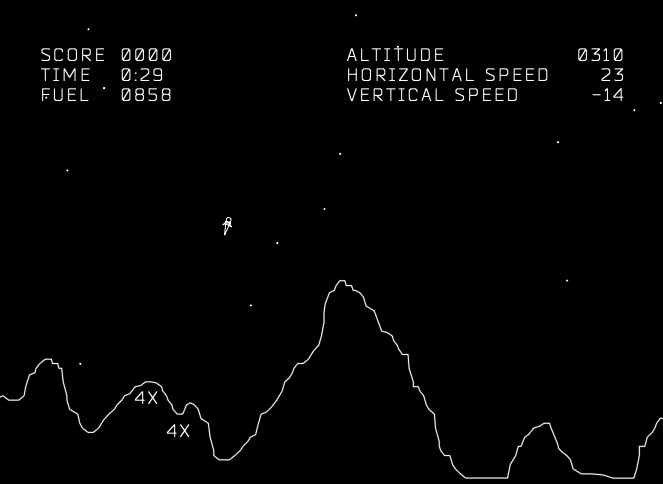
\includegraphics[width=200pt]{Figures/lunar_lander_gameplay.png}
    \caption{A screenshot from the``Lunar Lander'' Atari game. \cite{LunarLander}}
    \label{fig:gameplay}
\end{figure}

The optimal strategy for playing this game, as well as many other video games, has been thoroughly studied as a reinforcement learning problem. Viable solutions have been found using techniques such as actor-critic \cite{medium_RL} and Q-learning algorithms \cite{atari_RL}. Though there isn't much prior research into solving ``Lunar Lander'' using optimal control theory, the problem we are dealing with is reminiscent of real-world problems in aerospace engineering and space travel. The issue of autonomous landing is one that has been researched continuously over past decades, and optimal control has long-since been one of the most common approaches \cite{pinpoint_landing,nasa}. This field has seen major improvements in the past decade , including SpaceX's recent success in `catching' a descending rocket using automated landing control \cite{spacex}. In our simplified modeling of ``Lunar Lander'', we do not consider many real-world challenges such as the size of our lander and air resistance, just to name a couple. However, we hope that we can use the simplified assumptions given in the video game in order to find solutions that could generalize to more realistic situations.


\section{Mathematical Representation}
\label{sec:Math-Representation}
The game is two-dimensional, so only movement in the $x$ (horizontal) and $y$ (vertical) directions is allowed. As described before, during the game the lander is controlled by rotating the lander and then either engaging the thrust or not. To make the numerical solution more tractable, we make the simplifying assumption that the lander applies thrust directly horizontally and vertically through the controls $u_x$ and $u_y$, representing the horizontal and vertical acceleration respectively. We can then reconstruct the rotation angle $\theta$ (measured as the angle from vertical orientation) and magnitude of the acceleration $\tau$, as shown in Figure \ref{fig:controls}. Moreover, we define the state vector, evolution equations, and boundary conditions to be

\begin{align}\label{state_equation}
    \begin{aligned}
        \mathbf{x} &= \begin{bmatrix}
            x \\
            y \\
            \dot{x} \\
            \dot{y}
        \end{bmatrix} = \begin{bmatrix}
            x_1 \\
            y_1 \\
            x_2 \\ 
            y_2
        \end{bmatrix},  
        \quad \dot{\mathbf{x}} = \mathbf{f}(\mathbf{x}) =
        % \begin{bmatrix}
        %     \dot{x} \\
        %     \dot{y} \\
        %     \ddot{x} \\
        %     \ddot{y}
        % \end{bmatrix} = 
        \begin{bmatrix}
            x_2 \\
            y_2 \\
            u_x \\
            u_y - g
        \end{bmatrix}
    \end{aligned}, \qquad
    &
    \begin{aligned}
        x_1(0) &= x_0 \\
        y_1(0) &= y_0 \\
        x_2(0) &= v_0^{x} \\
        y_2(0) &= 0
    \end{aligned}
\end{align}

%$x_1 = x$, $x_2 = \dot{x}$, $y_1 = y$, and $y_2 = \dot{y}$ so that we have a first-order system of ODEs.
where $x_0$, $y_0$, and $v_0$ are the starting x-position, y-position, and x-velocity respectively, and $g$ is a gravitational constant representing the acceleration due to gravity in the moon's atmosphere. The boundary conditions come from the given starting conditions, and the fact that the initial vertical velocity is zero in the game. We also enforce the boundary condition $y_1(t_f) = 0$, which enforces that the lander will reach the ground at the end of its trajectory. This gives us a first-order system of ODE's.

In order to minimize the fuel expended during flight, we seek to minimize the magnitude of the control, $\|\mathbf{u}\|_2^2 = u_x^2 + u_y^2$. This is because the amount of fuel used should be proportional to the magnitude of the thrust. To minimize the time taken to land, and to minimize the magnitude of the final velocity, we let the final time $t_f$ be free and employ the Bolza form to create a final time penalty function $\phi(t_f, \mathbf{x}(t_f))$, given by
\begin{align}
\phi(t_f, \mathbf{x}(t_f)) = \gamma\ t_f + \beta\left(x_2(t_f)^2 + y_2(t_f)^2\right),
\end{align} 
where $\gamma > 0$ and $\beta > 0$ are constants corresponding to the final time cost and the cost of final velocity (hitting the ground too hard), respectively.

Now, our earliest tests of the model showed that one additional element was needed in order for our modeling to actually match the gameplay of ``Lunar Lander.''
Those early tests often had a rocket trajectory that passed underneath the moon surface (so $y_1(t) < 0$) before arriving at the endpoint condition $y_1(t_f) = 0$ with small final velocity. Thus, the rocket landed safely, but on the wrong side of the moon's surface. Because we are modeling a lunar lander and not the Underminer's shortest path, we determined that a modeling adjustment was necessary. Thus, in order to enforce the constraint that the rocket does not descent below the surface, we subtract $\min(0, y_1(t))$ inside the integral portion of the cost functional. If $y_1(t)$ becomes negative for any $t < t_f$, this will impose an extra penalty. 
Putting this all together, we obtain the following cost functional:

\begin{align}\label{cost-functional}
    J[u] = \int_{0}^{t_f} \left[\alpha \|\mathbf{u}\|_2^2 - \nu\min(0, y_1(t))\right] dt + \phi(t_f, \mathbf{x}(t_f)).
\end{align}
\vspace{0cm}

where $\alpha>0$ and $\nu>0$ are constants corresponding to the cost of acceleration and the cost of the lander hitting the ground prematurely, respectively. 

% Using $g$ as a gravitational constant, the state equations corresponding to this system are
% \begin{align}
%     \dot{x_1} &= x_2, & x_1(0) = x_0 \\
%     \dot{x_2} &= u_x, & x_2(0) = v_0 \\
%     \dot{y_1} &= y_2, & y_1(0) = y_0 \\
%     \dot{y_2} &= u_y - g, & y_2(0) = 0,
% \end{align}

\section{Solution}\label{solution}

The Hamiltonian for the system is

\begin{align}
    H = p_1 x_2 + p_2 y_2 + p_3 u_x + p_4(u_y - g) - \alpha \|\mathbf{u}\|_2^2 + \nu\min(0, y_1(t)).
\end{align}

Next, we apply Pontryagin's Maximum Principle to obtain the necessary conditions for the optimal control.

The condition that $\dot{\mathbf{p}}= -\frac{D H}{d \mathbf{x}}$ gives the costate equations
\begin{align}
    \dot{p}_1 &=0  & \dot{p}_3 = -p_1 \\[1ex]
    \dot{p}_2 & = \nu h(-y_1) & \dot{p}_4 = -p_2
\end{align}

where $h$ is the Heaviside function. The condition $\frac{D H}{D \mathbf{u}} = 0$ then gives
\begin{align}
    p_3 - 2 \alpha u_x &= 0 & p_4 - 2 \alpha u_y &= 0 \\
    \implies u_x &= \frac{p_3}{2\alpha} & \implies u_y &= \frac{p_4}{2\alpha}
\end{align}
as the optimal control values.

Next, because $x_1$, $x_2$, and $y_2$ are all free at $t_f$, the conditions that $\mathbf{p}(0) = \frac{D \phi }{D \mathbf{x}}$ and $\mathbf{p}(t_f)= -\frac{D \phi }{D\mathbf{x}(t_f)}$ give the equations
\begin{align}
    p_1(t_f) & = 0 & p_3(t_f) = -2\beta x_2(t_f)\\[1ex]
    p_2(t_f) & = \text{free} & p_4(t_f) = -2\beta y_2(t_f).
\end{align}

Note that we do not have any endpoint conditions on $p_2$ because $y_1$ is fixed at both endpoints.
Finally, because we are optimizing over the final time $t_f$ as well, we have the condition $H(\tilde{t}_f) = \frac{\partial \phi }{\partial t}(\tilde{t}_f)$, giving

\begin{align}
    H(\tilde{t}_f) &= \gamma.
\end{align}

\section{Results and Interpretation}
Using the above solution, we first solve the simplest version of our problem. In the subsections that follow, we then consider additional layers of complexity by modifying the cost functional, discussing the accompanying changes to the conditions
% . Throughout this section, we will address situations that require 
% modifications to the cost functional and variations to the solution
derived in the previous section, and interpreting the results.
Rather than completely rederiving the corresponding evolution equations at each step, we use the same process given in section \ref{solution} above, showing the final results along with numerical estimates of solutions.

\subsection{The Simplest Problem}
The simplest case involves the cost function described in Equation (\ref{cost-functional}). We make the simplifying assumptions that the surface of the moon is completely flat, and we also neglect the fact that we want the lander to reach the ground right-side up (rotation angle $\theta$ close to 0). These additions will be treated more fully in Subsections \ref{subsec:Terrain} and \ref{subsec:landing-angle}. Therefore, the lander can touch down at any angle and at any point on the surface, so long as the magnitude of its final velocity is small enough to land safely.

We combined the state $\mathbf{x}$ and costate $\mathbf{p}$ into a single eight-element array, then passed the corresponding ODE system into \texttt{solve\_bvp}. An initial guess for the solution is required for \texttt{solve\_bvp}, and the initial guess we used for each of the variables is summarized below:
\begin{enumerate}
    \item $x_1$: Since $x_1(t_f)$ is free, a constant initial guess of $x_0$.
    \item $y_1$: An \texttt{np.linspace} ranging from $y_0$ to $0$, since $y_1(t_f) = 0$
    \item $x_2$:  An \texttt{np.linspace} ranging from $v_0$ to $0$, since we expect the velocity to approach 0 over time.
    \item All other variables: All 1's, because this was the most numerically stable option.
\end{enumerate}
% Our initial cost functional did not include the term $\nu \min{(0, y_1(t))}$ that is shown in the previous section, and did not prevent the lander from reaching a negative vertical position. Because of this, many of our first attempts at solving for the optimal control produced trajectories that involved the rocket dropping slightly below the moon's surface, then slowly rising and coming to a stop on the ground. %TO DO: Maybe put a plot of this?
% Obviously, this is not a feasible option for a moon lander, so we adjusted the cost function to penalize any trajectory that takes the lander below ground level.

After rectifying the sub-surface trajectory issue mentioned in Section \ref{sec:Math-Representation}, we experimented with values for $\alpha$, $\beta$, $\gamma$, and $\nu$ and produced realistic solutions for this simplest case. We note here that all of our solutions obtained using \texttt{solve\_bvp} were highly dependent on small changes in initial conditions. An example of a successful lander trajectory is given in Figure \ref{fig:trajectory}. We found that the horizontal velocity starts at $x_0$ and decreases steadily to zero, while the vertical velocity starts at zero, decreases as the rocket moves downwards, and then goes back up toward zero for a soft landing. We also see that $\theta$ starts towards the left to counter the initial velocity and  moves towards zero (upright) over time, and the magnitude of the acceleration increases over time to slow the rocket down before it lands. See Figure~\ref{fig:controls} for plots of these results.

\begin{figure}[h]
    \centering
    \begin{subfigure}{0.45\textwidth}
        \centering
        % 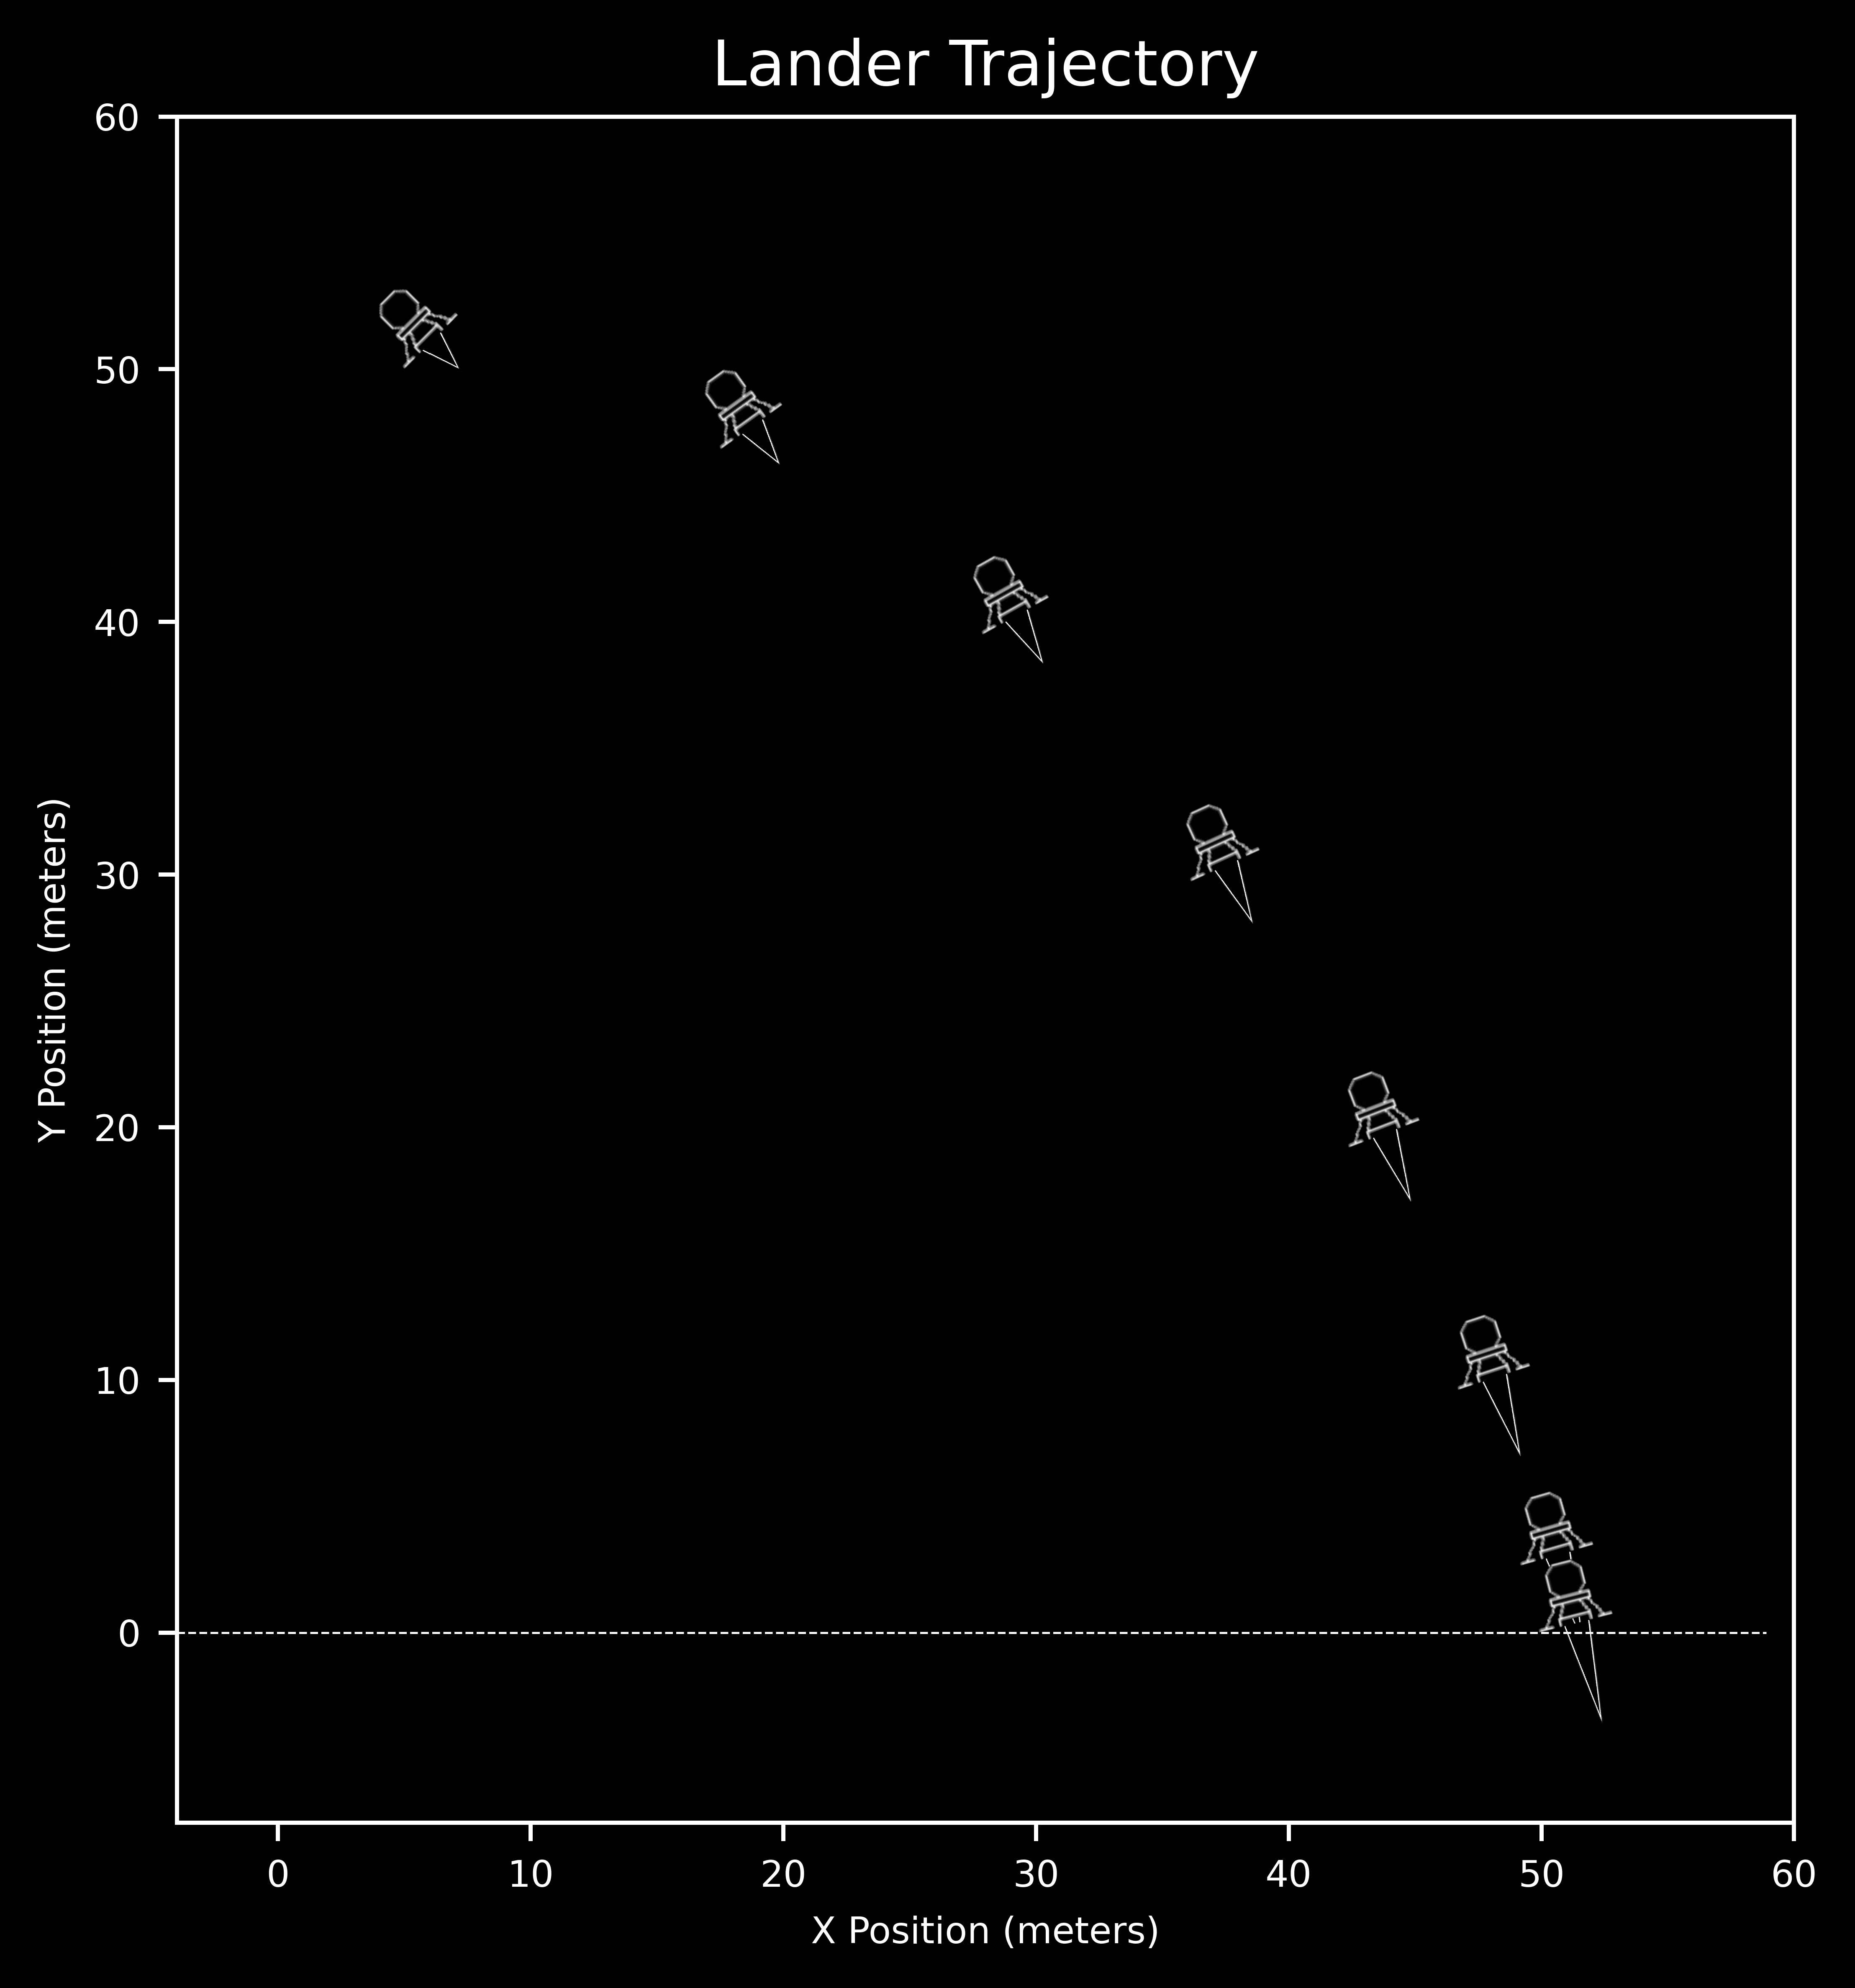
\includegraphics[width=\linewidth]{Figures/trajectory.png}
        \raisebox{0.13\height}{ % Adjust this value as needed
        \includegraphics[width=\linewidth]{Figures/boring_baseline_timelapse.png}
        }
        \caption{The optimal trajectory for a lander descending on a flat surface. (Lander image from \cite{reddit_media_2025})}
        \label{fig:trajectory}
    \end{subfigure}
    \hfill
    \begin{subfigure}{0.45\textwidth}
        \centering
        \includegraphics[width=\linewidth]{Figures/boring_baseline_results_v2.png}
        \caption{The velocities and controls corresponding to the optimal trajectory.}
        \label{fig:controls}
    \end{subfigure}
    \caption{The solution to the simplified version of ``Lunar Lander.''}

\end{figure}

\subsection{Landing with Terrain}
\label{subsec:Terrain}
In the game, rather than having a flat landing surface, the moon's surface is made up of jagged mountains and valleys. In order to descend safely, the lander must avoid any jagged terrain and touch down on a flat portion of the moon's surface. In this subsection, we explore different methods of simulating an uneven landing surface.
% \begin{enumerate}
%     \item Landing on Flat Ground: The rocket can only land safely on a flat area. Rather than defining which parts of the terrain are “flat enough,” we designate a specific horizontal position, known to be flat, as the target landing site. The rocket must land precisely at this location.
%     \item Avoiding Mountains: Since the moon’s surface is uneven, the rocket must avoid colliding with high terrain. To manage this, we define the vertical position $y_1 = 0$ as the lowest point of the surface. The rocket's trajectory must remain above the terrain throughout the descent.
% \end{enumerate}


\subsubsection{Landing at a Fixed Target}
First, we consider the scenario where the lander is given a set of predetermined target coordinates for landing. This might occur in the game, where the entire landscape is visible from the start, or in a more real-world situation where the landing surface is well-studied enough to give a known safe position for landing. Two different approaches to this are described below.
% We use both constraints and endpoint costs to obtain this objective.
\begin{enumerate}
    \item We directly constrain the lander’s final position by imposing the boundary condition
    \begin{align*}
        x_1(t_f) = x_f
    \end{align*}
    for some fixed value of $x_f$. This method is simple to implement because the cost functional and Hamiltonian remain unchanged, and we simply replace the costate boundary condition $p_1(t_f)=0$ with the state boundary condition $x_1(t_f) = x_f$. Making this adjustment gave results that were very similar to the basic, free endpoint case in terms of the solution's behavior. 
    \item Instead of enforcing an endpoint constraint, we modify the cost functional to penalize deviations from a given target position $x_f$:
    \begin{align*}
    J[u] = \int_{0}^{t_f} \left[\alpha \|\mathbf{u}\|_2^2 - \nu\min(0, y_1(t))\right] dt + \phi(t_f, \mathbf{x}(t_f)) + \mu (x_1(t_f) - x_f)^2.
    \end{align*}
    The additional term in the cost functional is weighted by some constant $\mu$ and increases as the final horizontal position moves away from the target. In this case, the transversality condition enforces a new boundary condition on the costate:
    \begin{align*}
    p_1(t_f) = 2 \mu (x_1(t_f) - x_f)
    \end{align*}
\end{enumerate}

We evaluated both techniques and found that enforcing a fixed endpoint position generally yielded more consistent results in terms of landing at the correct horizontal location.
However, this often came at the expense of other key factors—such as final velocity, landing angle, and even vertical position, with the rocket sometimes descending below the surface.
While failing to land in the target zone is a losing condition, so is violating these other constraints.
Conversely, when we relied solely on a soft cost penalty to encourage landing at the target position—rather than enforcing it—the rocket often failed to reach the correct horizontal spot, landed at steeper angles, and sometimes even passed below the surface.
These issues were especially evident in cases where the positional penalty became too weak relative to the other cost components.
In Figure \ref{fig:low_a}, Method 2 successfully landed in the correct horizontal location when using lower values for $\alpha$ and $\gamma$, and higher values for $\nu$ and $\mu$.
While Method 1 also landed correctly, it did so with a relatively steep angle.
Figure \ref{fig:regular} demonstrates, with default values for $\alpha$ and $\gamma$ and a lower value of $\mu$, that Method 2 failed to produce a viable solution, while Method 1 succeeded with a similar trajectory as produced by the previous set of parameters.
An interesting behavior we observed in both methods was that, when a target endpoint was specified, the rocket often initially accelerated away from the target before adjusting its trajectory and drifting back toward the landing point.
This suggests the optimizer was leveraging additional time or space to correct its path under tight constraints.
\begin{figure}[h]
    \centering
    \begin{subfigure}{0.45\textwidth}
        \centering
        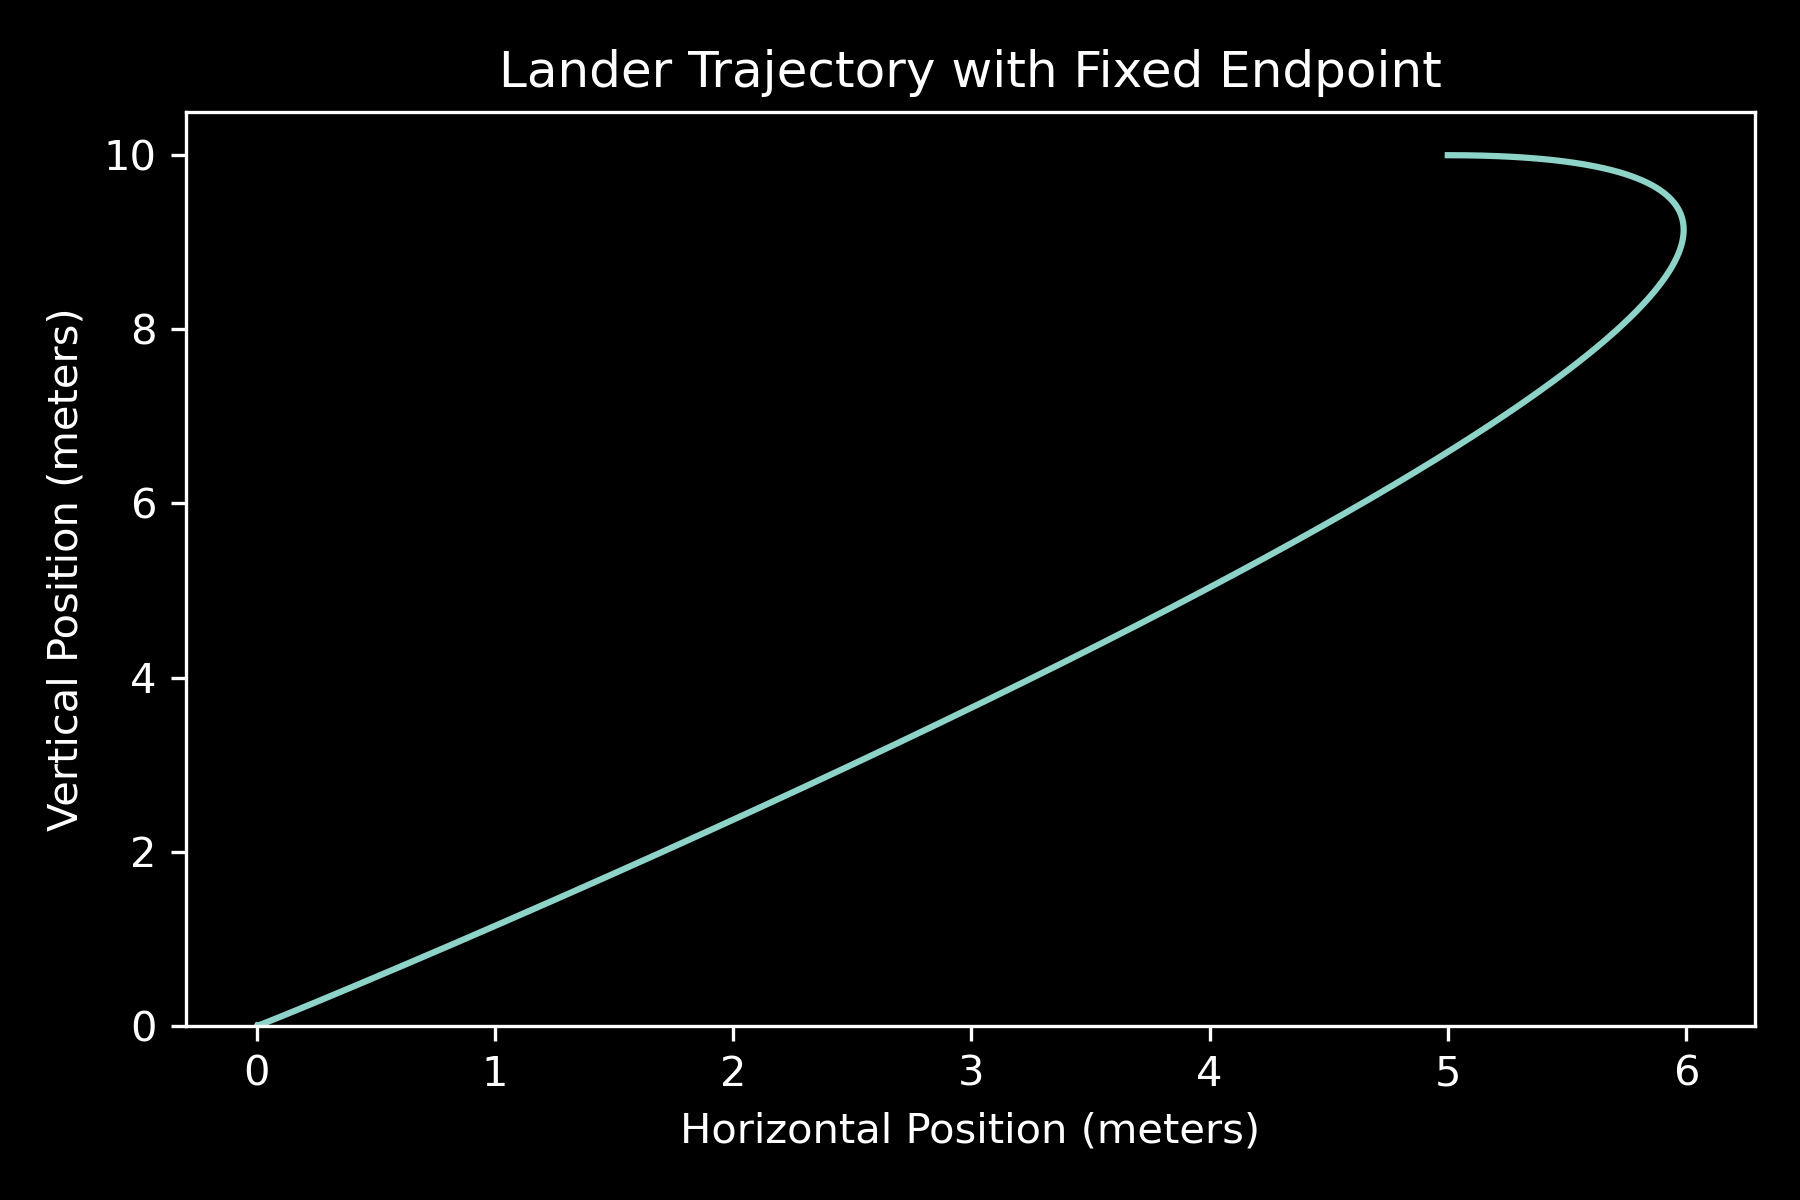
\includegraphics[width=\linewidth]{Figures/good_fixed_endpoint.png}
        \caption{Optimal Trajectory using Method 1.}
        \label{fig:Cost Successful}
    \end{subfigure}
    \hfill
    \begin{subfigure}{0.45\textwidth}
        \centering
        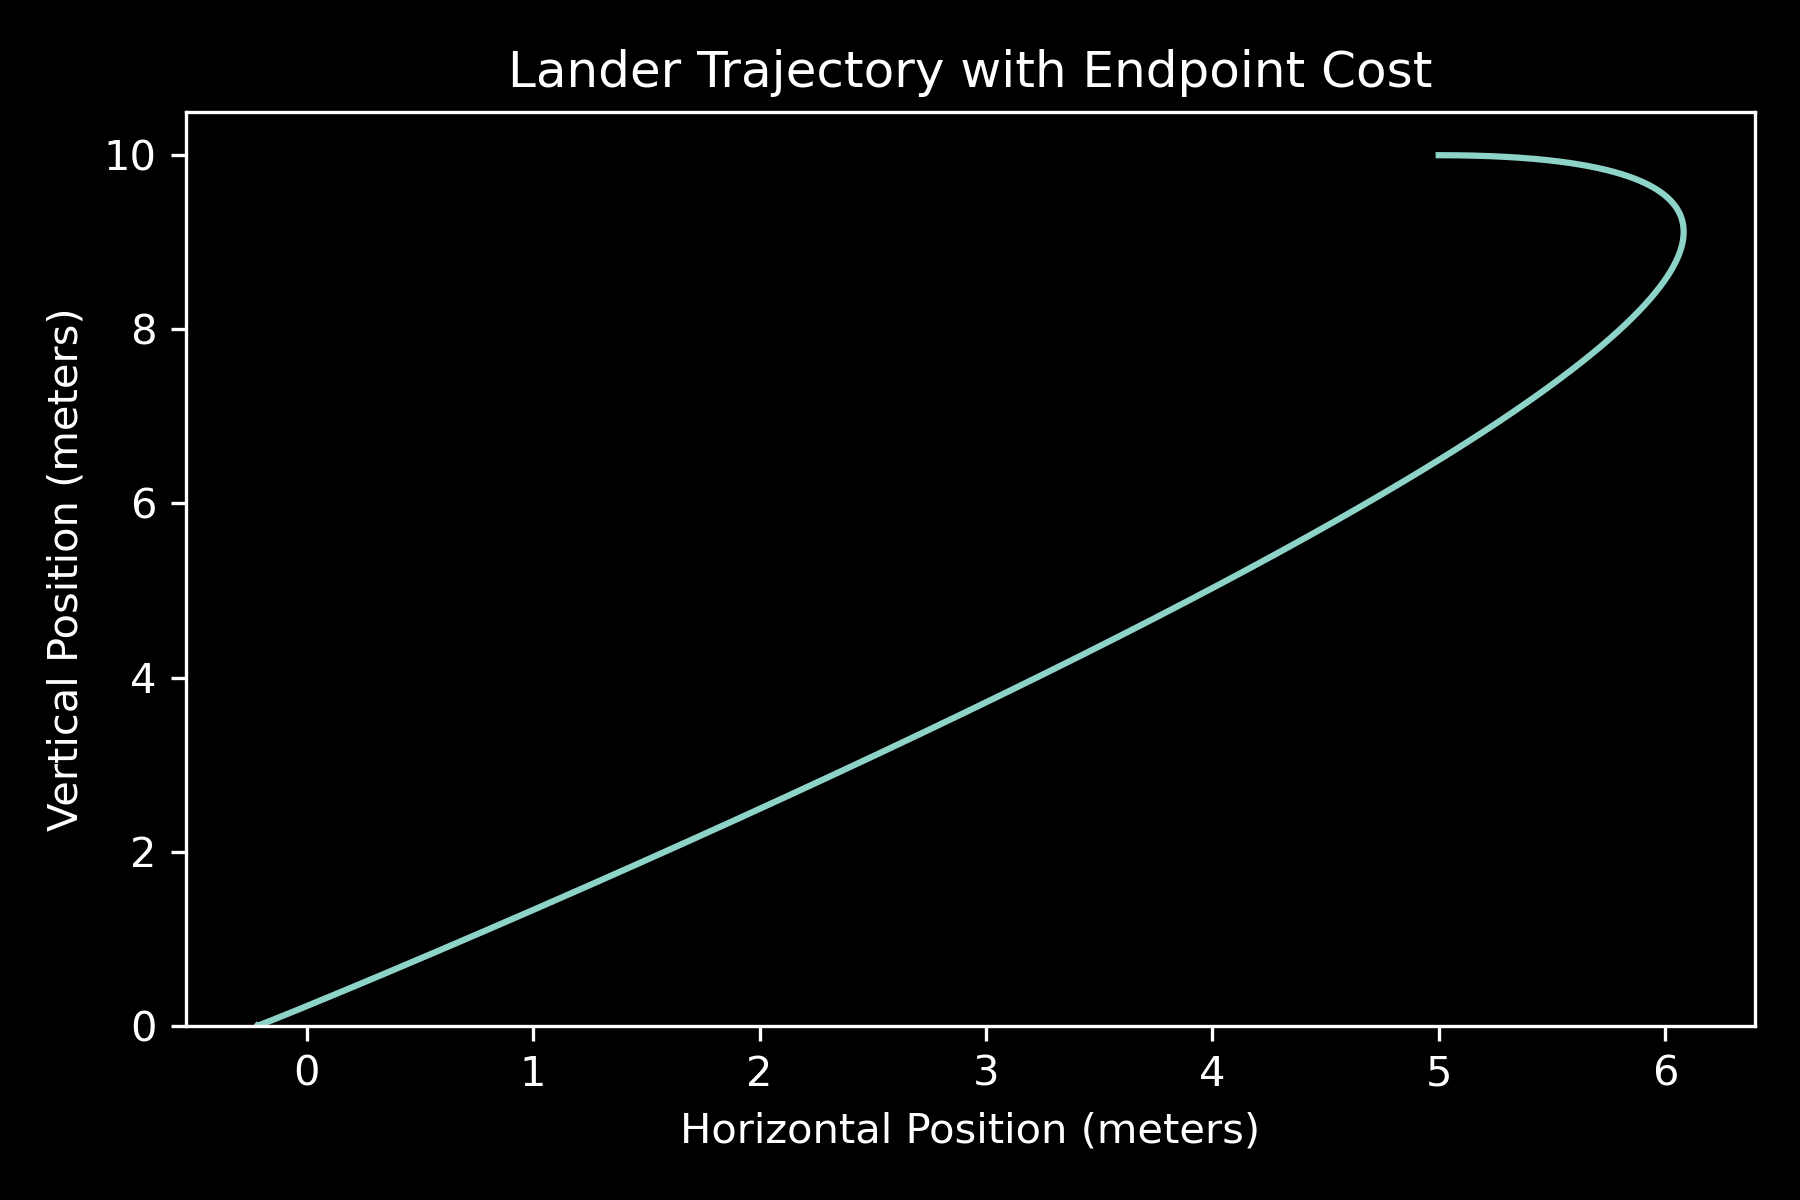
\includegraphics[width=\linewidth]{Figures/good_endpoint_cost.png}
        \caption{Optimal trajectory using Method 2.}
        \label{fig:Condition 1}
    \end{subfigure}
    \caption{Trajectories of landers with the origin as the target landing point. Both use parameters $\alpha$ = 10, $\beta = 1000$, $\gamma$ = 3, $\nu$ = 40, and $\mu$ = 25. The landers appear to follow the same general path, but the trajectory produced using Method 2 lands slightly offset from the origin.}
    \label{fig:low_a}
\end{figure}
\begin{figure}[h]
    \centering
    \begin{subfigure}{0.45\textwidth}
        \centering
        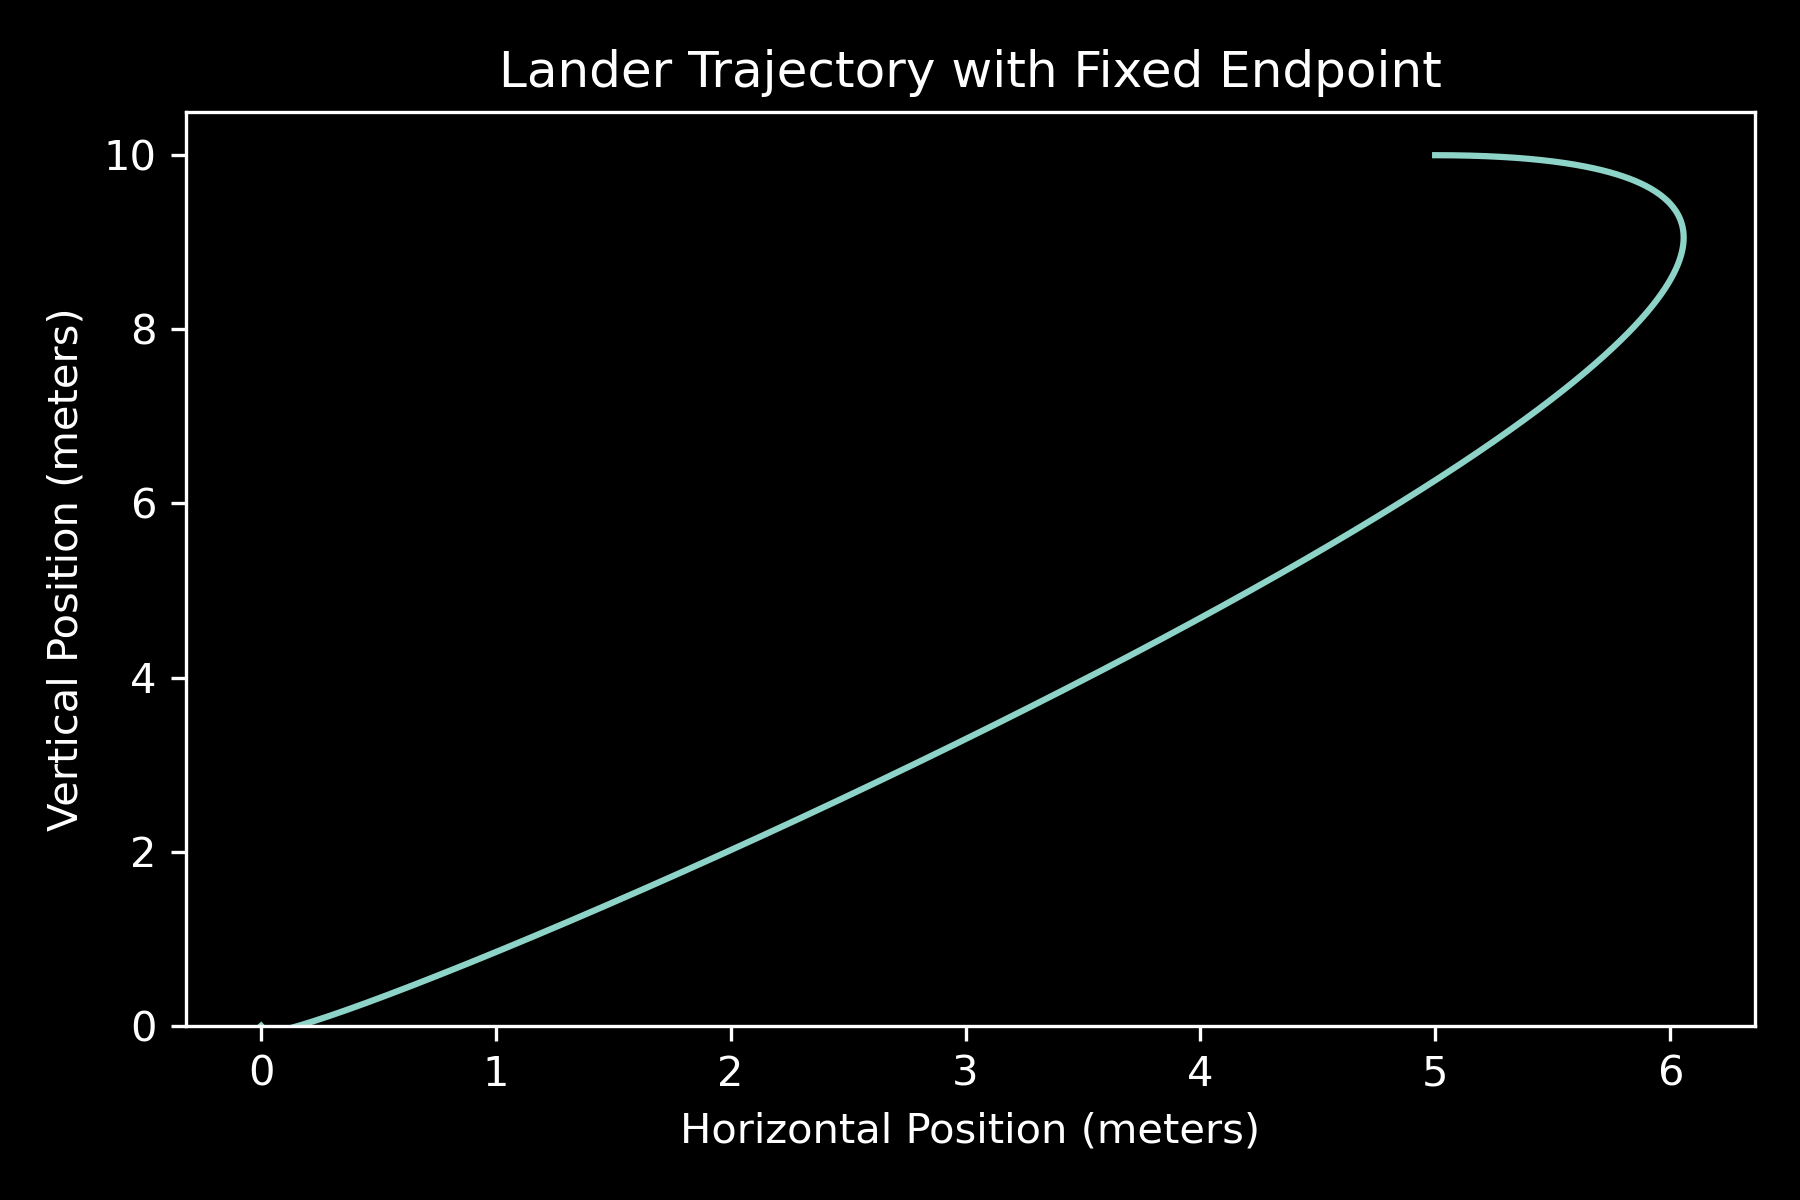
\includegraphics[width=\linewidth]{Figures/bad_fixed_endpoint.png}
        \caption{Method 1.}
        \label{fig:Cost Unsuccessful}
    \end{subfigure}
    \hfill
    \begin{subfigure}{0.45\textwidth}
        \centering
        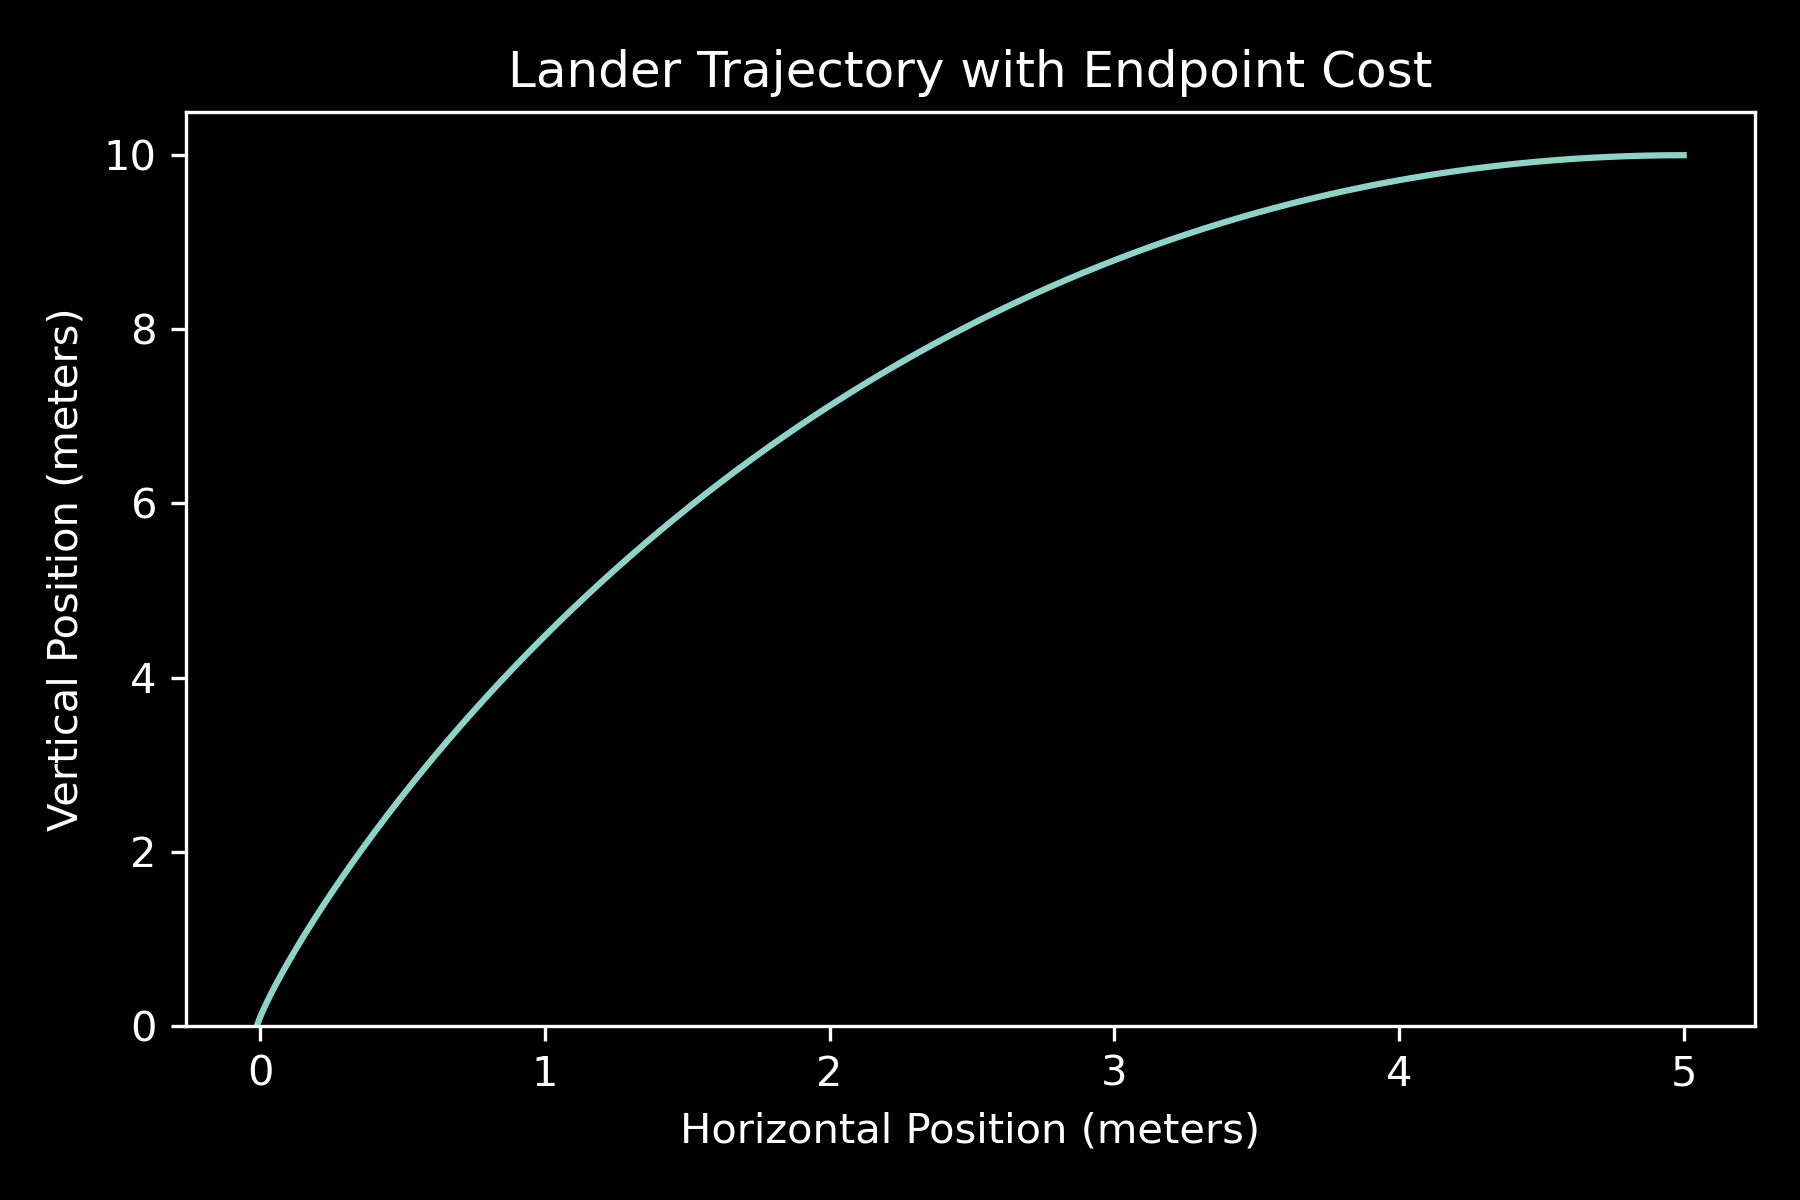
\includegraphics[width=\linewidth]{Figures/bad_endpoint_cost.png}
        \caption{Method 2.}
        \label{fig:Condition 2}
    \end{subfigure}
    \caption{Trajectories of landers with the origin as the target landing point. Both use parameters $\alpha$ = 15, $\beta = 100$ $\gamma$ = 15, $\nu$ = 40, and $\mu$ = 10. Although Method 2 appears to produce a good solution, this actually corresponds to a negative final time, which is impossible.}
    \label{fig:regular}
\end{figure}

Ultimately, using a hard constraint on the final position ensures that the rocket lands where intended, while relying on a soft penalty can lead to uncertainty in successfully reaching the target horizontal position. In Method 2, high values of $\mu$ often diluted the effect of the positional penalty, allowing the optimizer to prioritize other objectives, sometimes resulting in trajectories that dipped below the surface. Attempting to correct this by increasing the other constants, such as $\alpha$ or $\gamma$, frequently caused the rocket to miss the horizontal target altogether. This highlights the delicate balance required to tune the parameters for optimal performance.
\pagebreak
\subsubsection{Landing with Obstacle Avoidance}
In addition to the case where the lander is guided towards a specific target landing location, we also considered the situation where the lander may land anywhere on the moon's surface, but there are certain obstacles (mountains, craters, small asteroids, enemy star-bases, etc.) which the lander must avoid. That is, the lander may take any path and land in any location as long as it does not collide with the obstacles. In order to account for this in our optimal control problem, we must first represent these obstacles mathematically, then adjust our cost functional accordingly. For simplicity, we use the following function to represent obstacles as ellipses centered at $(c_x, c_y)$ with horizontal radius $r_x$ and vertical radius $r_y$:
\begin{align}
    C(x, y) = \frac{\lambda}{\left( \frac{(x - c_x)^2}{r_x} + \frac{(y - c_y)^2}{r_y} \right)^{20} + 1}.
\end{align} The constant $\lambda$ is a weight representing the penalty for the lander hitting the obstacle. Now, given a set of obstacles $\{C_1, ..., C_k\}$, we can modify the cost functional as follows:
\begin{align}
    J[u] = \int_{0}^{t_f} \left[\alpha \|\mathbf{u}\|_2^2 - \nu\min(0, y_1(t)) + \sum_{i=1}^{k}{C_i(x_1(t), y_1(t))} \right] dt + \phi(t_f, \mathbf{x}(t_f)).
\end{align}
This change to the cost functional gives the new Hamiltonian
\begin{align}
    H = p_1 x_2 + p_2 u_x + p_3 y_2 + p_4(u_y - g) - \alpha \|\mathbf{u}\|_2^2 + \nu\min(0, y_1(t)) - \sum_{i=1}^{k}{C_i(x_1(t), y_1(t))}
\end{align}
as well as the corresponding costate evolution equations 
\begin{align}
    \dot{p}_1 &= \sum_{i=1}^{k}{C_x^i(x_1, y_1)}  & \dot{p}_3 = -p_1 \\[1ex]
    \dot{p}_2 & = \sum_{i=1}^{k}{C_y^i(x_1, y_1)} + \nu h(-y_1) & \dot{p}_4 = -p_3.
\end{align}
The boundary conditions remain the same as in the basic (no obstacles, free endpoint) scenario.
This scenario proved much more difficult to solve numerically than the ones discussed previously. 
Initial modeling of the obstacle avoidance scenario produced optimal trajectories that traveled well below the moon's surface, traveled backwards in time, and collided with obstacles multiple times. 
% TO DO: include a few plots of these fails
The most effective, though very challenging, solution that we found to this issue was finding a suitable balance of all of the weights in the cost functional. Because every obstacle may have a unique weight $\lambda_i$, there are $k+4$ weights to specify, and varying any one of them by even a few tenths led to drastically different results. After much trial and error, we found the following general guidelines that (most of the time) produce desirable solutions:
\begin{itemize}
    \item The value of $\nu$ should be significantly larger than all other weights. This is because descending below the moon's surface in a lander is impossible.
    \item The same weight should be applied to all conditions that result in a crash. That is, both colliding with an obstacle and hitting the ground with too great a velocity will cause the lander to explode, and therefore we should set $\beta = \lambda_i$ for all $i$. We found that if any of these are not equal, the solution will essentially ignore the less-weighted component(s). This results in solutions that pass directly through obstacles or essentially free fall to the surface.
    \item The more obstacles and components there are, the smaller $\alpha$ and $\gamma$ need to be. This is essentially saying that if we want to be more specific about where we land and the path we take, we need to be more lenient about fuel usage and flight duration. Using larger values for either of these weights again results in solutions that either ignore obstacles or approach the surface too quickly.
\end{itemize}
All of our successful solutions in obstacle avoidance were produced using weights $\nu = 40$, $\beta = \lambda_i = 25$, and $\alpha, \gamma \leq 1$. 
We also found, as before, that solutions to the obstacle avoidance scenario are very sensitive to different initial guesses. While we used a straight vertical drop as the initial guess in most previous cases, this did not produce good results for obstacle avoidance. In order to find an optimal path that avoids all obstacles, the initial guess must also avoid all obstacles. However, this does not mean that the optimal solution will follow a similar trajectory to the initial guess. In fact, the solution would often travel in the opposite direction as the initial guess (see Figure \ref{initial_guesses}). Determining conditions for a suitable initial guess, as well as constructing an initial guess that avoids given obstacles, is an interesting topic for further study.

% \begin{figure}[h]
%     \centering
%     \begin{subfigure}{0.32\textwidth}
%         \centering 
%         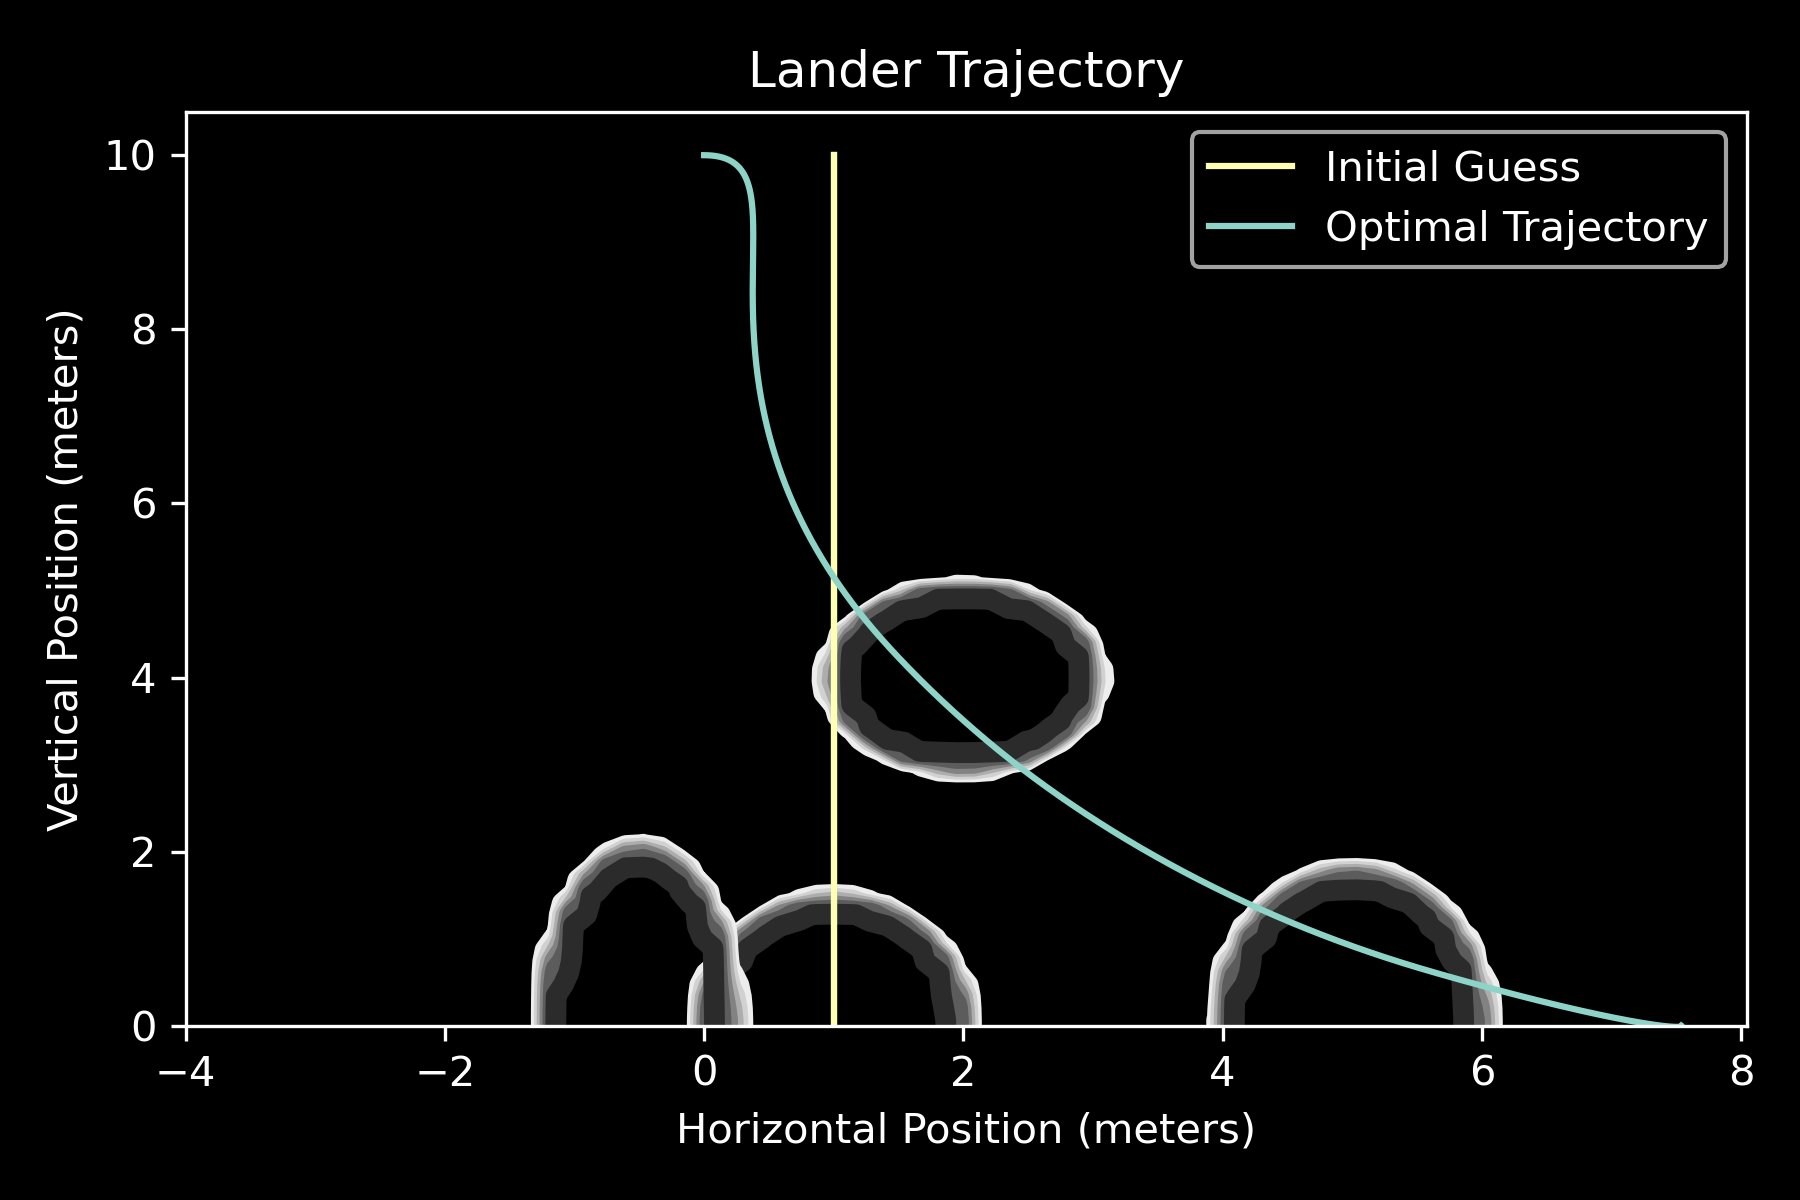
\includegraphics[width=\linewidth]{Figures/obstacle_init_guess_3.png}
%     \end{subfigure}
%     \begin{subfigure}{0.32\textwidth}
%         \centering 
%         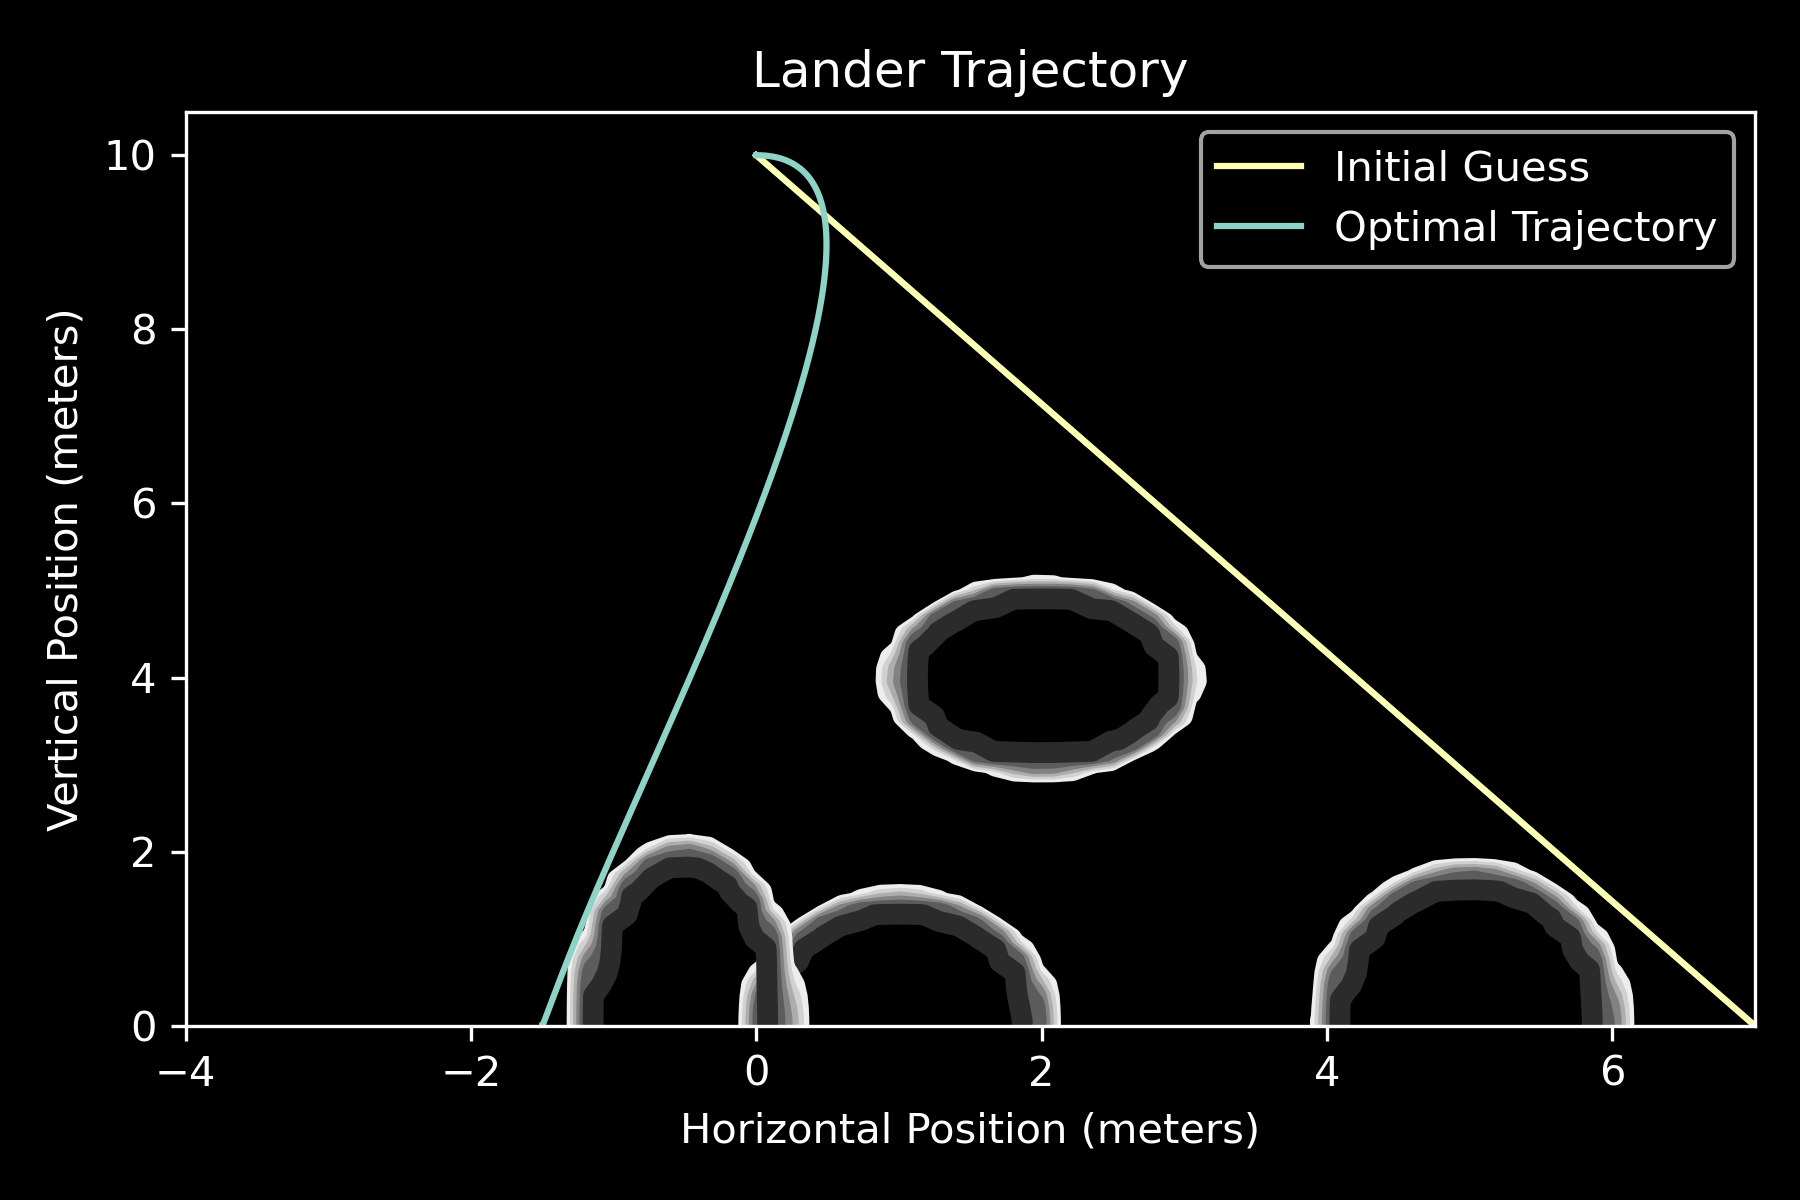
\includegraphics[width=\linewidth]{Figures/obstacle_init_guess_1.png}
%     \end{subfigure}
%     \begin{subfigure}{0.32\textwidth}
%         \centering 
%         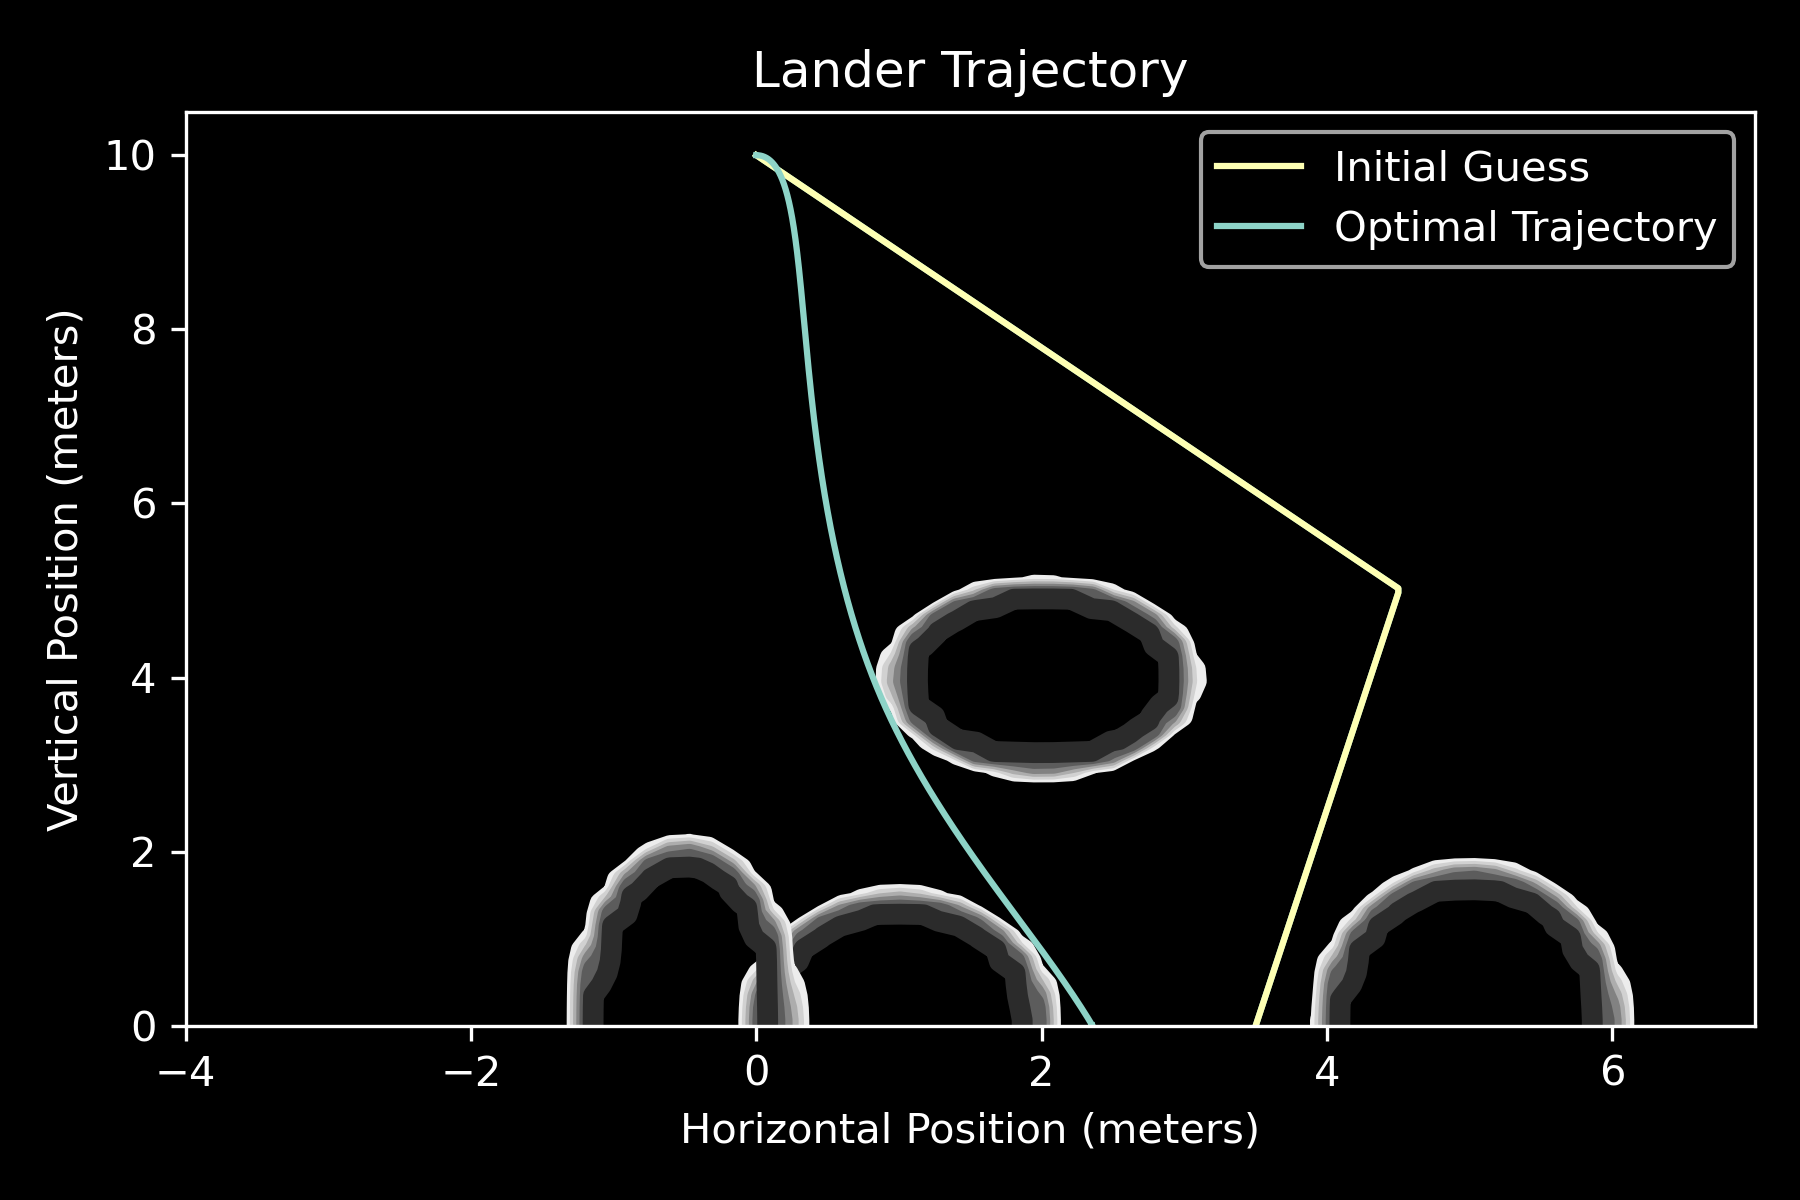
\includegraphics[width=\linewidth]{Figures/obstacle_init_guess_2.png}
%     \end{subfigure}
%     \caption{Three ``optimal'' trajectories to the same obstacle avoidance problem. Each plot is generated with a different initial guess passed to \texttt{solve\_bvp}. The rightmost plot produced the best solution in terms of duration and low landing velocity, with landing time $t_f = 2.4953$. However, this solution used much more fuel than the trajectory shown in the center plot.}
%     \label{initial_guesses}
% \end{figure}

\begin{figure}[hbt]
    \centering

    % Top row
    \begin{subfigure}{0.45\textwidth}
        \centering 
        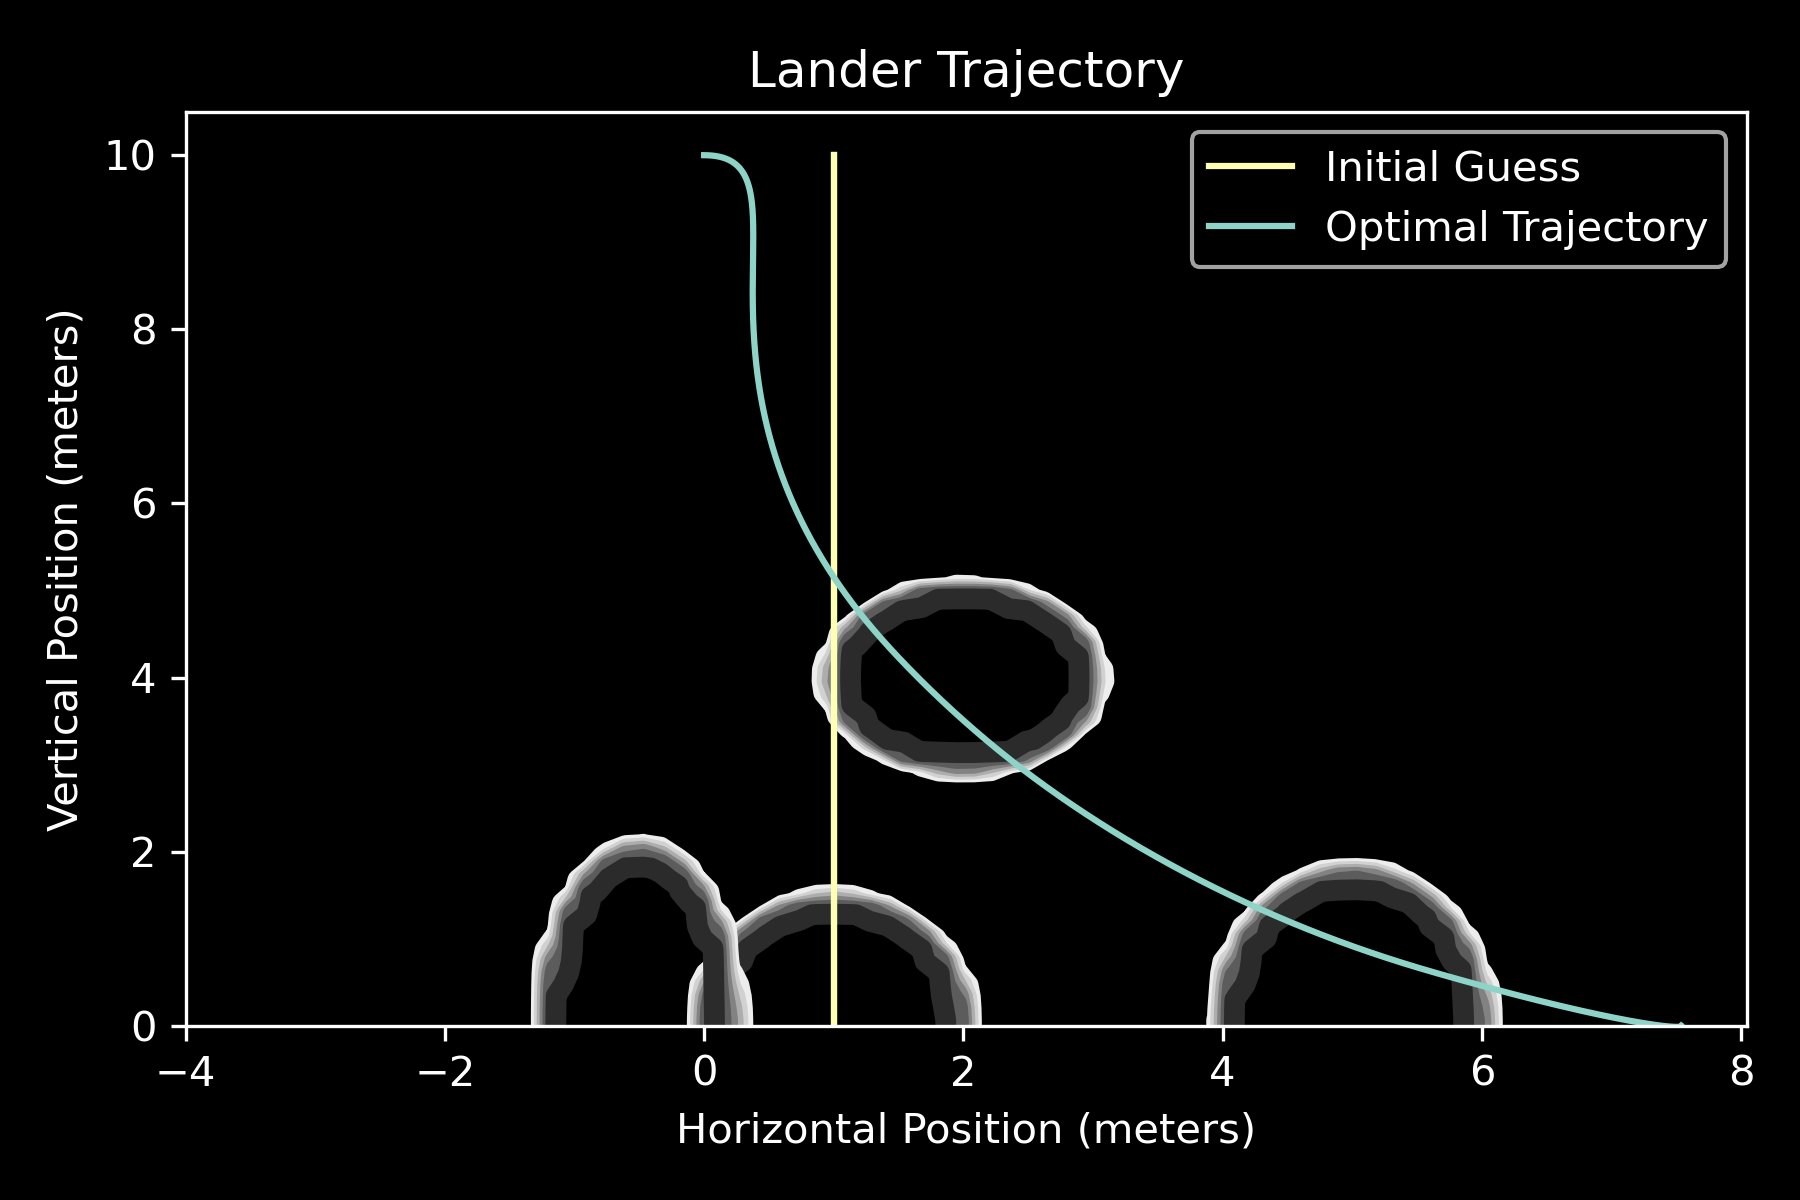
\includegraphics[width=\linewidth]{Figures/obstacle_init_guess_3.png}
        \caption{}
    \end{subfigure}
    \hspace{0.05\textwidth}
    \begin{subfigure}{0.45\textwidth}
        \centering 
        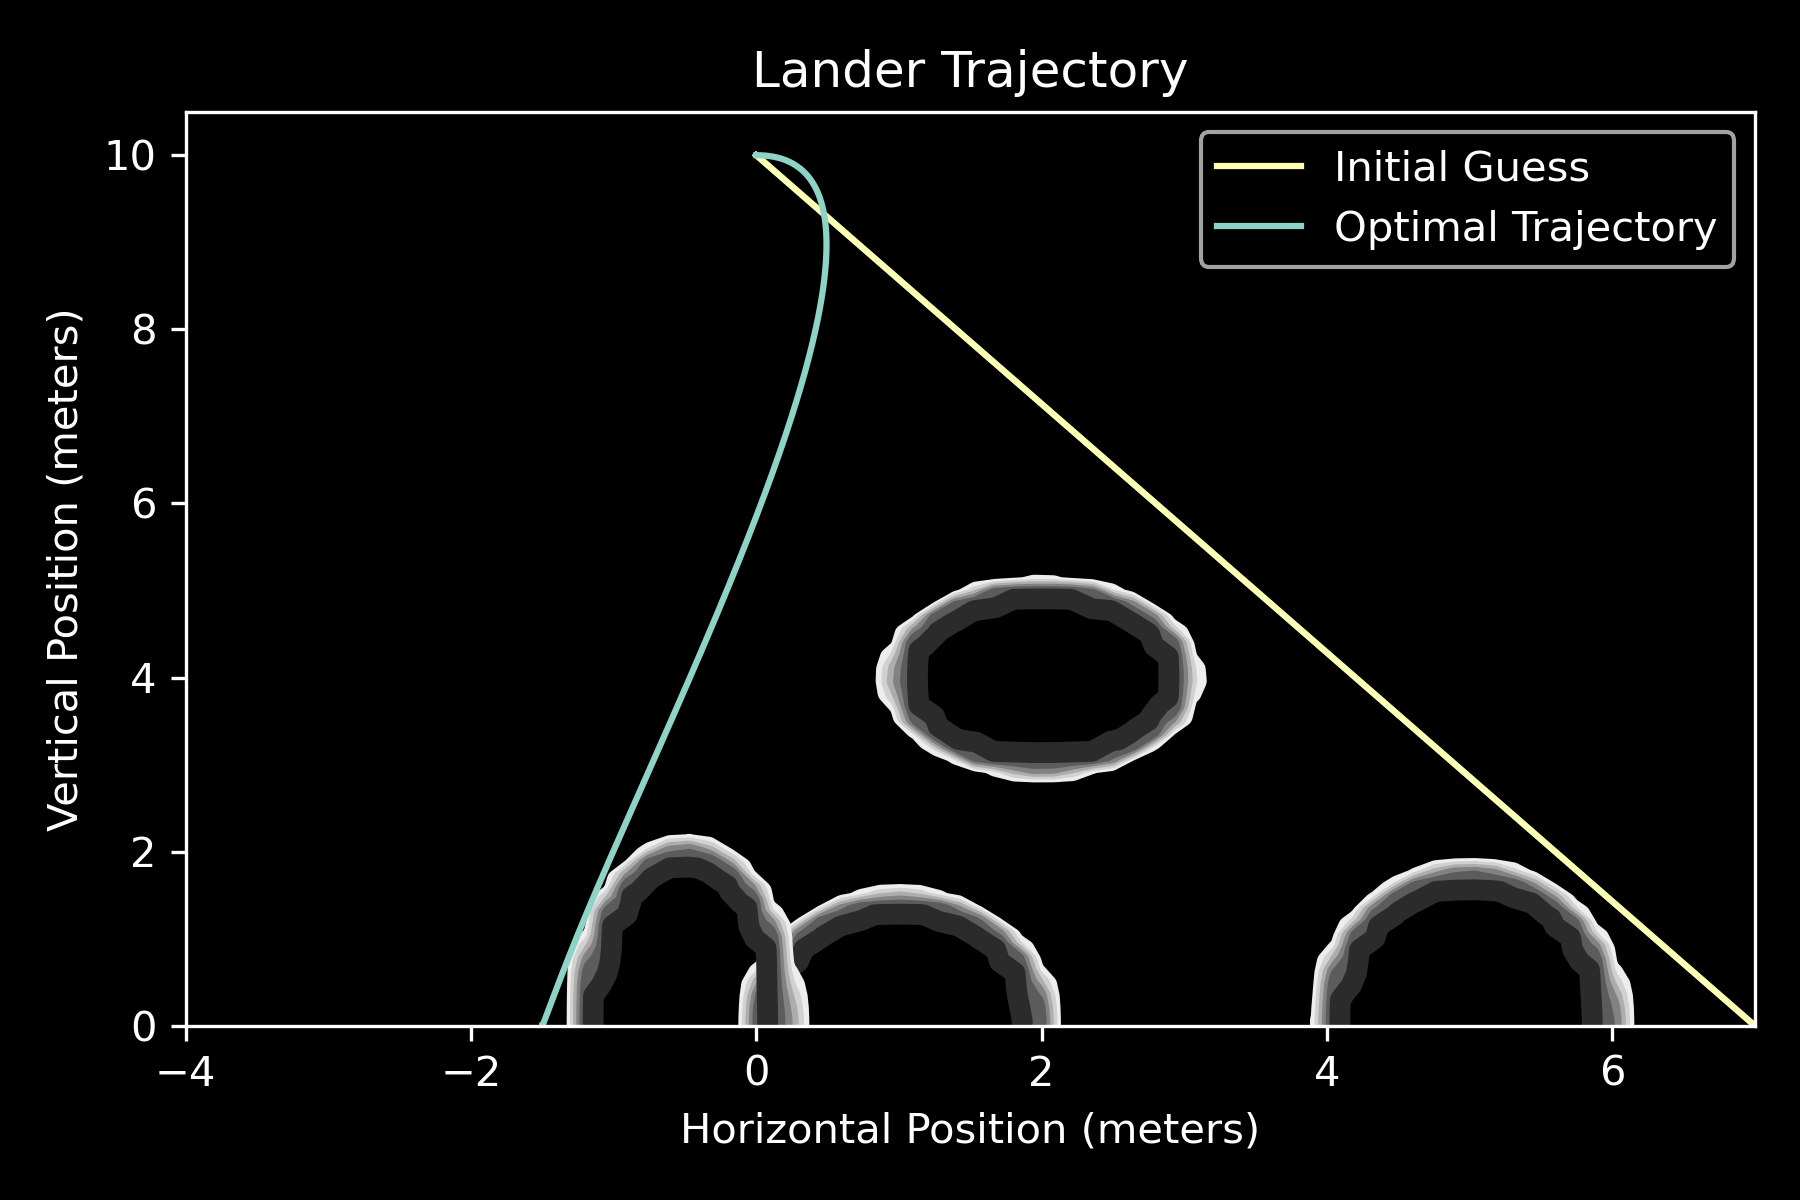
\includegraphics[width=\linewidth]{Figures/obstacle_init_guess_1.png}
        \caption{}
    \end{subfigure}

    \vspace{0.5cm}

    % Bottom row - same width, centered
    \begin{subfigure}{0.45\textwidth}
        \centering 
        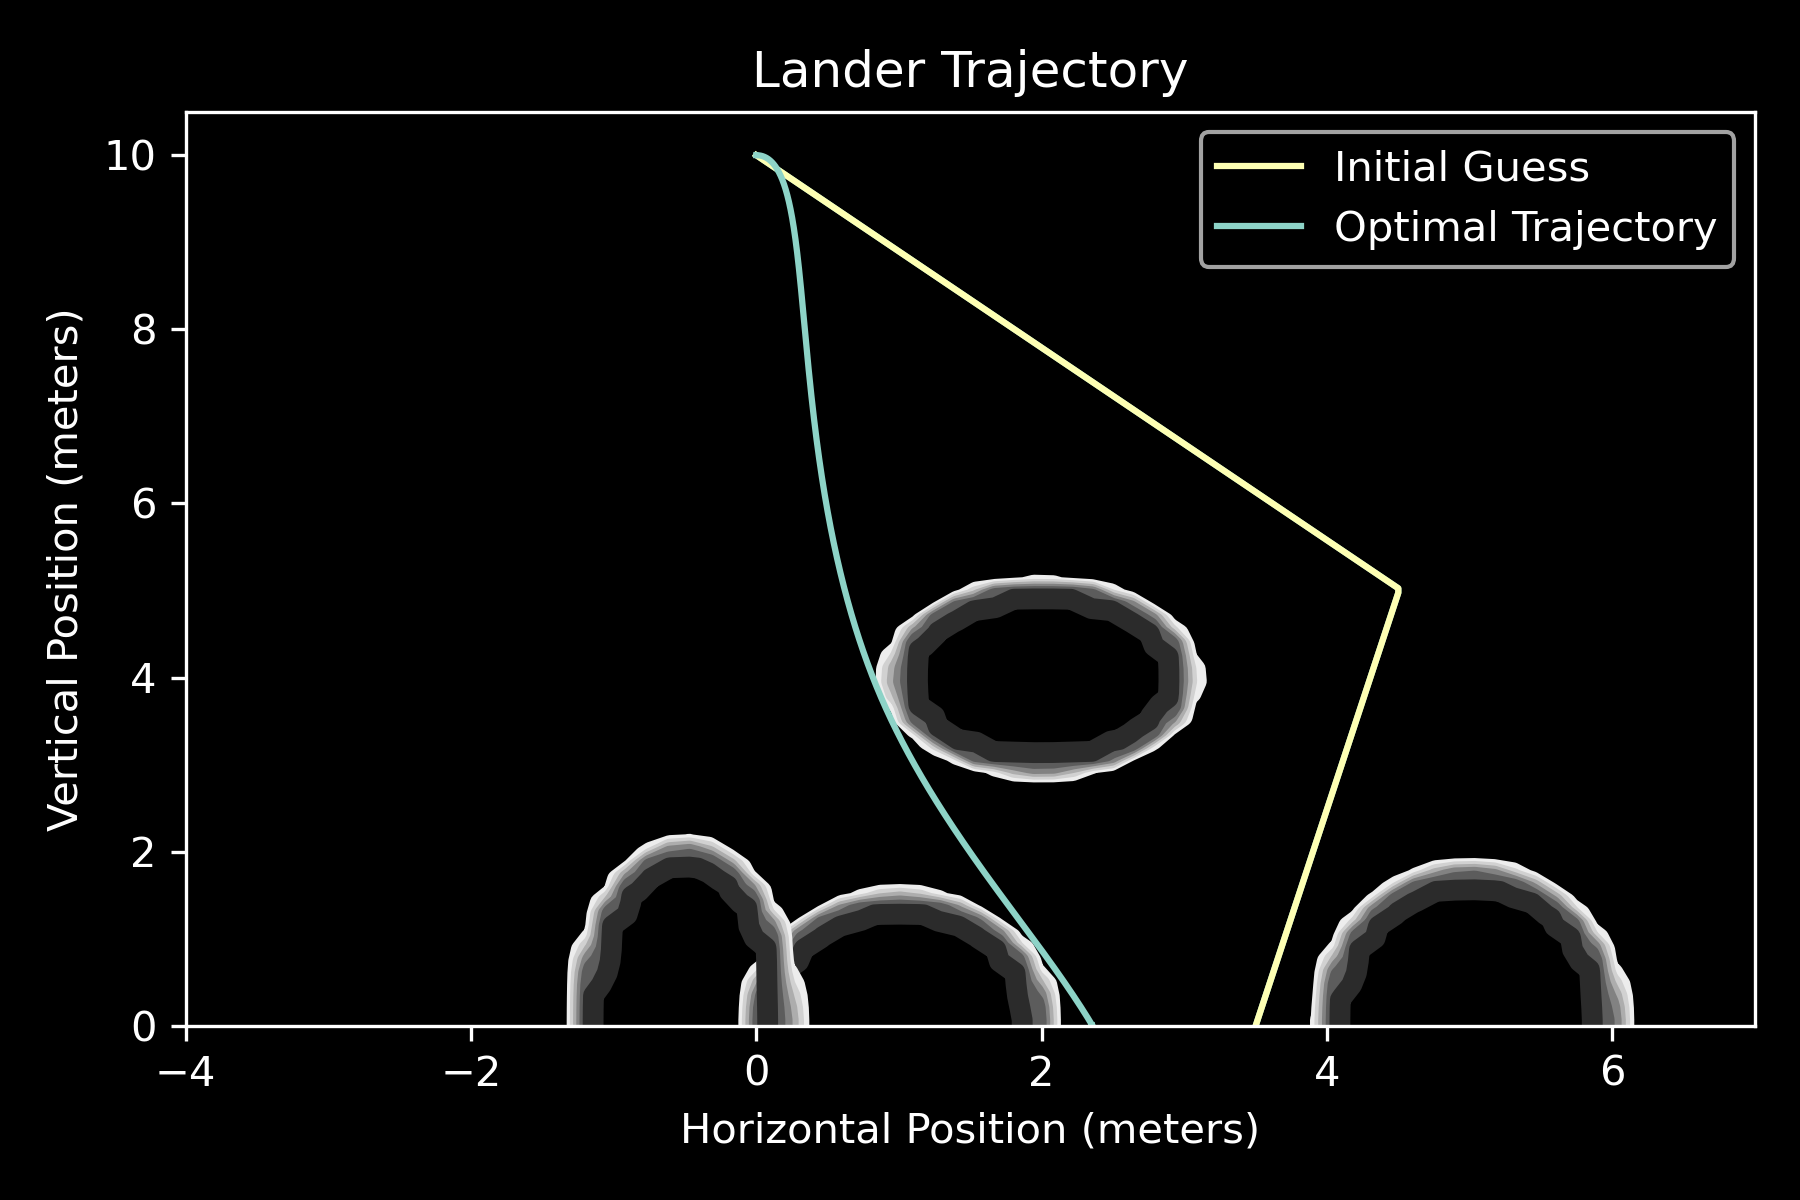
\includegraphics[width=\linewidth]{Figures/obstacle_init_guess_2.png}
        \caption{}
    \end{subfigure}

    \caption{Three ``optimal'' trajectories to the same obstacle avoidance problem. Each plot is generated with a different initial guess passed to \texttt{solve\_bvp}. Plot (c) produced the best solution in terms of duration and low landing velocity, with landing time $t_f = 2.4953$. However, this solution used much more fuel than the trajectory shown in plot (b). \\
    Note: The obstacles are graphed as contour plots, where the actual body of the obstacle is the dark interior, and the gray to white border represents a margin of decreasing penalty around the obstacle. So, while the lander appears to scrape the surface of some obstacles in plots (a) and (b), it actually skirts around the obstacles with a narrow margin.}
    \label{initial_guesses}
\end{figure}



One other point of concern we encountered in obstacle avoidance was numerical instability. In many cases we encountered runtime and divide-by-zero errors, and some solutions that appear to have smooth trajectories actually correspond to controls that fluctuate rapidly and have discontinuities. Analyzing the numerical stability of solving this problem presents another valuable area for future research.

\pagebreak
\subsection{Minimizing the Landing Angle}
\label{subsec:landing-angle} 
To successfully land in the game, the lander must be upright ($\theta \approx 0$) when it arrives at the ground (time $t_f$). The methods we have learned in Volume 4 only pertain to penalizing/constraining final values of the state $\mathbf{x}(t_f)$, not the control $\mathbf{u}$. While this may be possible, it was outside the scope of this project, so we sought to address this issue by instead minimizing $|\theta|$ so that $\theta\approx0$, where $\theta$ is reconstructed from the controls as $\theta = \text{arctan}(\frac{-u_x}{u_y})$. 
% We set out to implement this part of the game into our cost functional, but ran into the following question: how do we penalize final control values? In class we only talked about penalizing final values of the state, while it might be possible to control the final value of the control, this was outside the scope of the class and therefore attempted to address the problem in another way. Instead, we desired to minimize the $|\theta| = |\text{arctan}(\frac{-u_x}{u_y})|$ so that $\theta\approx0$ (which means the rocket is upright). 
This implies that we want $|u_x|\approx0$ as $y_1(t)\rightarrow0$ so that $\frac{-u_x}{u_y}\approx0$ no matter the value of $u_y$.
% because even if $u_y\ll1$ (which would cause $\frac{-u_x}{u_y}$ to be very large) we still have $\frac{-u_x}{u_y}=0$. Thus we wanted $|u_x|\approx0$ as $y_1(t)\rightarrow0$. 
To implement this, we experimented with the following two methods:
\begin{enumerate}
    \item First, we modify the cost function to penalize $u_x$ as $y_1(t)\rightarrow0$ as follows:
    \begin{align}
    J[u] = \int_{0}^{t_f} \left[\alpha \|\mathbf{u}\|_2^2 - \nu\min(0, y_1(t)) + \left(\frac{u_x}{y_1(t) + \rho}\right)^2\right] dt + \phi(t_f, \mathbf{x}(t_f)) 
    % + \mu u_y,
    \end{align}
    Here, $0<\rho <1$ is included to avoid division by zero as $y_1(t)\rightarrow0$. The idea behind the $(\frac{u_x}{y_1 + \rho})^2$ term is that as $y_1(t)$ gets smaller than 1, the cost on $u_x^2$ begins to be magnified so it is penalized more the closer the lander gets to the ground. We allowed $\rho$ to vary to allow us to tune the resulting solutions.  
    % because we weren't sure what would happen, and we wanted to avoid numerical instability. 
    This results in the following changes to the Hamiltonian and costate, while everything else remains the same:
    \begin{align}
    H = p_1 x_2 + p_2 y_2 + p_3 u_x + p_4(u_y - g) - \alpha \|\mathbf{u}\|_2^2 + \nu\min(0, y_1(t)) - \left(\frac{u_x}{y_1(t) + \rho}\right)^2
    \end{align}
    \begin{align}
    \dot{p}_2 & = \nu h(-y_1)  + 2\frac{u_x^2}{(y_1(t) + \rho)^3}
    \end{align}
    Unfortunately, this implementation made $\theta$ approach $\pi$ or $-\pi$ because $u_y$ was not constrained, which was not what we expected.
    % This was our motivation for Subsection \ref{subsec:KKT}.
    % which makes sense because those are viable options if $u_y$ isn't constrained.
    \item Second, 
    % because we were skeptical of our results from the first method, 
    we tried to penalize $|u_x|$ using a method similar to our treatment of the sub-surface solutions in Section \ref{sec:Math-Representation} with the parameter $\nu$. We modified the cost function as follows:
    \begin{align}
    J[u] = \int_{0}^{t_f} \left[\alpha \|\mathbf{u}\|_2^2 - \nu\min(0, y_1(t)) - \zeta\min(0, y_1(t) - \epsilon)u_x^2\right] dt + \phi(t_f, \mathbf{x}(t_f))
    \end{align}
    Here, $\epsilon > 0$, $\zeta > 0$. Essentially, once $y_1(t)$ comes within $\epsilon$ of the moon surface, $u_x^2$ starts to be penalized, with $\zeta$ being the adjustable penalty. 
    This results in the following changes to the Hamiltonian and costate while everything else remains the same:
    \begin{align}
    H = p_1 x_2 + p_2 y_2 + p_3 u_x + p_4(u_y - g) - \alpha \|\mathbf{u}\|_2^2 + \nu\min(0, y_1(t)) +  \zeta\min(0, y_1(t)-\epsilon)u_x^2
    \end{align}
    \begin{align}
    \dot{p}_2 & = \nu h(-y_1)  + \zeta h(-y_1(t)+\epsilon)u_x^2.
    \end{align}
    Unfortunately, this solution had similar results to first method, where $\theta$ approached $\pi$ or $-\pi$.
\end{enumerate}
We believe this is because we do not have and inequality constraint $u_y > 0$. Without this constraint, $\text{arctan}(\frac{-u_x}{u_y})$ easily goes to $\pi$ or $-\pi$ because of the way that \texttt{np.arctan2()} treats negatives, even if $u_x=0$. These results became our motivation for Subsection \ref{subsec:KKT}.

\subsection{Adding Control Constraints}
\label{subsec:KKT}
To address the limitations discussed in the previous section, we also sought to constrain the vertical control $u_y$ to prevent the lander from accelerating down.
Obviously, gravity already causes the lander to accelerate downwards, but we want to avoid having the lander turn over and propel itself downwards more quickly.
Specifically, this motivates the constraint
\begin{align*}
    -u_y \leq 0.
\end{align*}
We do this because
1) in the game, the lander is not allowed to propel itself downwards, exhibited by the fact that the lander cannot rotate past horizontal,
% and must always be oriented upward
and 
2) we generally care more about preserving fuel than minimizing time.

Applying this constraint along with the addition from the previous subsection gives the new optimal control problem of minimizing
\begin{align}
    J[u] = \int_{0}^{t_f} \left[\alpha \|\mathbf{u}\|_2^2 - \nu\min(0, y_1(t)) - \zeta\min(0, y_1(t) - \epsilon)\right] dt + \phi(t_f, \mathbf{x}(t_f)) + \mu u_y
\end{align}
subject to
\begin{align}
    \mathbf{x}' &= \mathbf{f}(\mathbf{x}), \\
    -u_y &\leq 0, \quad \mu \geq 0, \quad u_y \mu = 0, \label{kkt_cont}
\end{align}
where $\mathbf{f}$ is from Equation~(\ref{state_equation}).
In this case, our state and costate equations remain unchanged, but now we have
\begin{align}
    \frac{D \mathscr L}{D u_x} &= p_3 - 2\alpha u_x + 2\zeta \min(0, y_1(t) - \epsilon)u_x = 0, \\
    \frac{D \mathscr L}{D u_y} &= p_4 - 2\alpha u_y + \mu = 0.
\end{align}
From these, we obtain
\begin{align}
    u_x &= \frac{p_3}{2\left(\alpha - \zeta \min(0, y_1(t)-\epsilon)\right) } \quad \text{and} \quad u_y = \frac{p_4 + \mu }{2\alpha },
\end{align}
and applying the third KKT condition from Equation (\ref{kkt_cont}) we have either $\mu = 0$ or $\mu = -p_4$.
However, after applying these to our numerical method, the results are quite poor.
To see exactly how poor, view Figure~\ref{fig:bad_trajectory} in the Appendix.
% the interpretation and results section to see the numerical estimates.

\section{Conclusion}

\subsection{Summary Results}
After many adjustments and lots of fine-tuning, most of our models produced solutions that were realistic and reflect the controls and trajectories that we had expected. We hypothesized that the lander would drift in the direction of its initial velocity, increasing the magnitude of its thrust as it descended in order to ensure a smooth landing. While the direction of the lander's descent varied in situations with a target landing zone or obstacles to avoid, the controls generally followed this expected trend. We produced viable optimal trajectories in many cases, and hypothesized general rules to produce suitable parameters and initial guesses for our optimal control problem. 
% \subsubsection{Using Methods of Landing at a Specified Ending Position}
% Overall, our results showed a high degree of instability. For both optimization methods, tuning the cost function constants proved challenging and often produced undesirable outcomes. When we adjusted the cost functional to penalize deviations from the target position, it tended to weaken the influence of other critical costs. In some cases, this caused the rocket to crash below the lunar surface. Furthermore, the positional penalty was sometimes not strong enough to guide the rocket to the desired landing area. Introducing an end condition for horizontal position did help the rocket land in the correct horizontal location more consistently. However, this came at the expense of other performance metrics: the final velocities, landing angle, vertical position, and duration of flight. In both approaches, the constants used in the cost function had a significant impact on the outcome and were very temperamental. Moving forward, we would benefit from a metric to evaluate landing success based on angle, time, velocity, and final position. With such a metric in place, we could systematically explore constant values to identify an optimal combination for our functional and constraints.
With regards to our results on the penalizing the angle and trying to use KKT to restrict $u_y$ where mostly poor results. In fact, some of our initial models that used the baseline model (that didn't consider final angle  or the inequality constraint on $u_y$) seemed to have had more realistic plots for $\theta$, the angle of the rocket.


\subsection{Challenges}
One of the primary challenges we encountered was that our initial model produced unrealistic trajectories where the lander dipped below the lunar surface before ascending to land. While mathematically valid due to the endpoint condition being met, such behavior was clearly infeasible in practice. To address this, we modified the cost functional to penalize negative vertical positions, which improved realism but introduced new difficulties in tuning the corresponding weight. 
% Additionally, the model proved extremely sensitive to the choice of constants in the cost functional. Small changes in weights like $\alpha$, $\beta$, or $\nu$ would frequently lead to drastically different trajectories—ranging from crashing into obstacles to violating time or fuel constraints (even solutions with negative final time were observed). 
Numerical instability posed another significant hurdle, particularly in the obstacle avoidance scenarios, where poorly chosen initial guesses often led to convergence failures or invalid solutions such as negative final time or discontinuous control values. These challenges required iterative tuning, model refinement, and careful construction of initial conditions to produce physically meaningful solutions.

Aside from the numerical instability of our problem, we also found it very difficult to balance the weights of the different components of our cost functional. This is demonstrated in our modeling of endpoint targets. When we adjusted the cost functional to penalize deviations from the target position, it tended to weaken the influence of other critical costs. In some cases, this caused the rocket to crash below the lunar surface. Furthermore, the positional penalty was sometimes not strong enough to guide the rocket to the desired landing area. Introducing an end condition for horizontal position did help the rocket land in the correct horizontal location more consistently. However, this came at the expense of other performance metrics: the final velocities, landing angle, vertical position, and duration of flight. In both approaches, the constants used in the cost function had a significant impact on the outcome and were very temperamental. 

\subsection{Future Research Directions}
Throughout this project, we made numerous simplifying assumptions that made the modeling process more clear and easy to work with, but also less realistic and less accurate to the ``Lunar Lander'' game. Undoing these simplifications and working our results into their original context presents a valuable area for future study. For example, in our derivation we made the assumption that the lander applies acceleration directly in the $x$ and $y$ directions, while the game allows the player to first set an angle for the lander, then apply thrust in that direction. It would be interesting to model the same problem using these canonical values of angle and thrust magnitude as the controls. Building this model would likely require linearization around the lander's current position. In addition to our simplification in the controls, we use a minimum in our cost functional to force the lander's $y$ position to be nonnegative. We realized only after our modeling and analysis that this creates concerns for the theoretical solution to our optimal control problem, specifically because Pontryagin's Maximum Principal requires the derivative of the Lagrangian to be continuous, but adding a minimum function creates a discontinuity at $y_1=0$. This method still produced good results when solved numerically, and we hypothesize that this is because we are really only interested in the region where $y_1 > 0$, and the derivative of the Lagrangian is continuous on this region. However, given more time, we would like to explore other methods, such as adding slack variables to the state equation, that could prevent the trajectory from going below the surface without introducing discontinuity into the Lagrangian. In addition, more modeling could be done in order to transition this problem from the video game scenario into a real-world scenario. Part of this process could include moving from two to three dimensions, incorporating air resistance into our functional, or accounting for time delay in the application of controls.

Additionally, because of the difficulty in setting the hyperparameters of the model, we would benefit in the future from having a metric to evaluate landing success based on angle, time, velocity, and final position. With such a metric in place, we could systematically explore constant values to identify an optimal combination for our functional and constraints.
Other areas for future research stem from the difficulties that arose when applying numerical solvers to our optimization problem. Namely, we have discussed the challenges in determining the weights of the cost function and constructing a good initial guess, it would be interesting to look deeper into the details of numerical solving techniques in an attempt to put more strict ranges on the acceptable values for weights or initial guesses.

\newpage
\nocite{*}
\bibliographystyle{alpha}
\bibliography{writeup_references}

\newpage
\section{Appendix}
Here is one failed trajectory that illustrates some of the challenges we faced during implementation.

\begin{figure}[h]
    \label{fig:appendix}
    \centering
    \begin{subfigure}{0.45\textwidth}
        \centering
        % 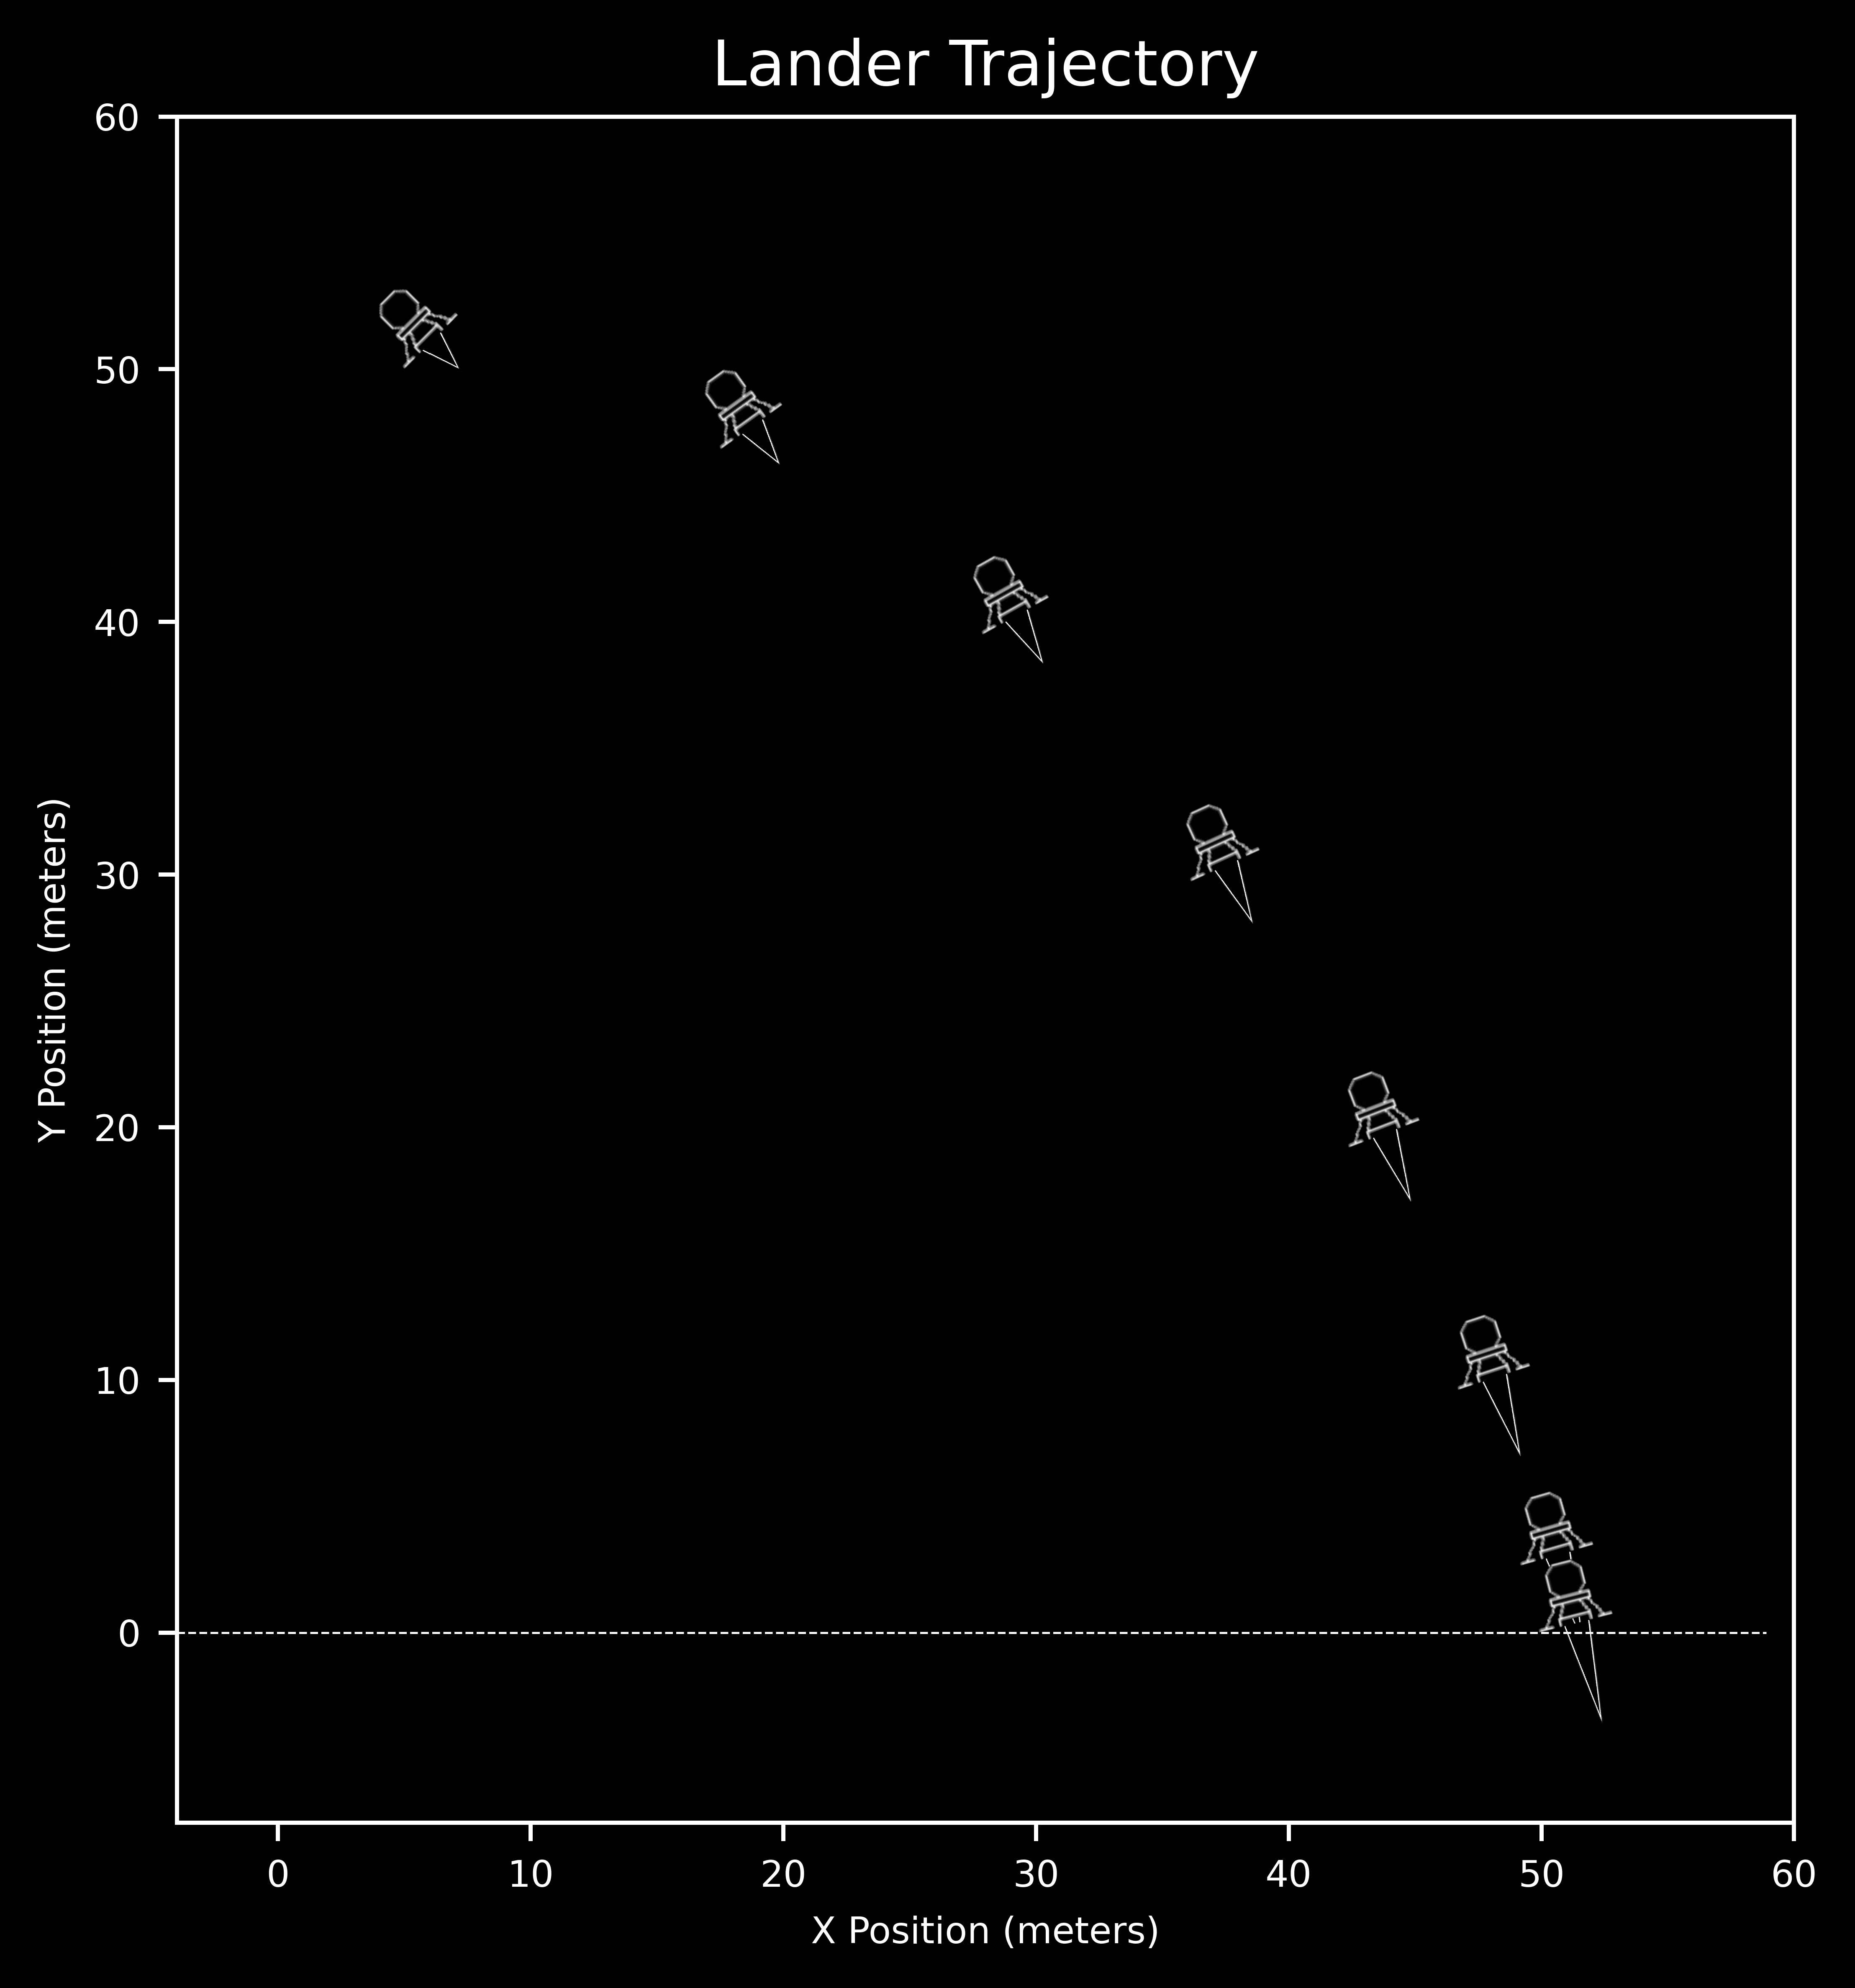
\includegraphics[width=\linewidth]{Figures/trajectory.png}
        \raisebox{1\height}{ % Adjust this value as needed
        \includegraphics[width=\linewidth]{Figures/bad_traj.png}
        }
        \caption{An ``optimal'' trajectory with $\zeta=100$, $\epsilon = 5$.}
        \label{fig:bad_trajectory}
    \end{subfigure}
    \hfill
    \begin{subfigure}{0.45\textwidth}
        \centering
        \includegraphics[width=\linewidth]{Figures/bad_traj_controls.png}
        \caption{Note how $\theta$ approaches $\pi$ instead of approaching 0 over time, and how vertical velocity decreases over time (the lander does not hit the ground with velocity close to 0).}
        \label{fig:badder_controls}
    \end{subfigure}
    \caption{A failed solution implementing the $u_x$ minimization strategies of Subsection \ref{subsec:landing-angle}.}
\end{figure}
\end{document}